\documentclass[
11pt, % The default document font size, options: 10pt, 11pt, 12pt
%oneside, % Two side (alternating margins) for binding by default, uncomment to switch to one side
english, % ngerman for German
singlespacing, % Single line spacing, alternatives: onehalfspacing or doublespacing
%draft, % Uncomment to enable draft mode (no pictures, no links, overfull hboxes indicated)
%nolistspacing, % If the document is onehalfspacing or doublespacing, uncomment this to set spacing in lists to single
%liststotoc, % Uncomment to add the list of figures/tables/etc to the table of contents
%toctotoc, % Uncomment to add the main table of contents to the table of contents
%parskip, % Uncomment to add space between paragraphs
%nohyperref, % Uncomment to not load the hyperref package
headsepline, % Uncomment to get a line under the header
%chapterinoneline, % Uncomment to place the chapter title next to the number on one line
%consistentlayout, % Uncomment to change the layout of the declaration, abstract and acknowledgements pages to match the default layout
]{Thesis} % The class file specifying the document structure
\setcounter{tocdepth}{2}

\usepackage[utf8]{inputenc} % Required for inputting international characters
\usepackage[T1]{fontenc} % Output font encoding for international characters

\usepackage{mathpazo} % Use the Palatino font by default

\usepackage{tikz}
\usetikzlibrary{positioning, shapes.geometric, arrows}
\tikzstyle{startstop} = [rectangle, rounded corners, minimum width=3cm, minimum height=1cm, text centered, draw=black, fill=blue!5]
\tikzstyle{process}   = [rectangle, 				 minimum width=3cm, minimum height=1cm, text centered, draw=black, fill=blue!5]
\tikzstyle{decision}  = [diamond  , 				 minimum width=3cm, minimum height=1cm, aspect=2, text centered, draw=black, fill=blue!5]
\tikzstyle{function}  = [trapezium, trapezium left angle=70, trapezium right angle=110, minimum width=2cm, text width=2cm, minimum height=1cm, text centered, draw=black, fill=blue!5]

\usepackage{listings}
\usepackage{xcolor}
\lstdefinestyle{PythonSnippet}{
	backgroundcolor = \color[rgb]{0.95,0.95,0.92},
	commentstyle = \color[rgb]{0,0.6,0},
	keywordstyle = \color{magenta},
	numberstyle = \tiny\color[rgb]{0.5,0.5,0.5},
	stringstyle = \color[rgb]{0.58,0,0.82},
	basicstyle = \ttfamily\footnotesize,
	breakatwhitespace = false,
	breaklines = true,
	captionpos = b,
	keepspaces = true,
	numbers = left,
	numbersep = 5pt,
	showspaces = false,
	showtabs = false,
	tabsize = 2,
	showlines = true
}
\lstset{style=PythonSnippet}

\usepackage[backend=bibtex,style=ieee,natbib=true]{biblatex} % Use the bibtex backend with the ieee citation style
\addbibresource{Sources.bib}

\usepackage[autostyle=true]{csquotes} % Required to generate language-dependent quotes in the bibliography

% \usepackage{environ}
% \RenewEnviron{figure}{} %Uncomment to hide all figures
% \RenewEnviron{table}{} %Uncomment to hide all tables

%----------------------------------------------------------------------------------------
%	MARGIN SETTINGS
%----------------------------------------------------------------------------------------

\geometry{
	paper=a4paper, % Change to letterpaper for US letter
	inner=2.5cm, % Inner margin
	outer=3.8cm, % Outer margin
	bindingoffset=.5cm, % Binding offset
	top=1.5cm, % Top margin
	bottom=1.5cm, % Bottom margin
	%showframe, % Uncomment to show how the type block is set on the page
}

%----------------------------------------------------------------------------------------
%	THESIS INFORMATION
%----------------------------------------------------------------------------------------

\thesistitle{8-bit CPU Architecture in Minecraft} % Your thesis title, this is used in the title and abstract, print it elsewhere with \ttitle
\supervisor{{Dr. Thomas} \textsc{Preu}} % Your supervisor's name, this is used in the title page, print it elsewhere with \supname
\examiner{} % Your examiner's name, this is not currently used anywhere in the template, print it elsewhere with \examname
\degree{Matura } % Your degree name, this is used in the title page and abstract, print it elsewhere with \degreename
\author{Damian \textsc{O'Dell}} % Your name, this is used in the title page and abstract, print it elsewhere with \authorname
\addresses{} % Your address, this is not currently used anywhere in the template, print it elsewhere with \addressname

\subject{Computer Sciences} % Your subject area, this is not currently used anywhere in the template, print it elsewhere with \subjectname
\keywords{} % Keywords for your thesis, this is not currently used anywhere in the template, print it elsewhere with \keywordnames
\university{K+S | MNG Rämibühl} % Your university's name and URL, this is used in the title page and abstract, print it elsewhere with \univname
\department{Department of Computer Science} % Your department's name and URL, this is used in the title page and abstract, print it elsewhere with \deptname
\faculty{} % Your faculty's name and URL, this is used in the title page and abstract, print it elsewhere with \facname

\AtBeginDocument{
\hypersetup{pdftitle=\ttitle} % Set the PDF's title to your title
\hypersetup{pdfauthor=\authorname} % Set the PDF's author to your name
\hypersetup{pdfkeywords=\keywordnames} % Set the PDF's keywords to your keywords
}

\begin{document}

\frontmatter % Use roman page numbering style (i, ii, iii, iv...) for the pre-content pages

\pagestyle{plain} % Default to the plain heading style until the thesis style is called for the body content

%----------------------------------------------------------------------------------------
%	TITLE PAGE
%----------------------------------------------------------------------------------------

\begin{titlepage}
\begin{center}

\vspace*{.03\textheight}
{\scshape\LARGE \univname\par}\vspace{1.5cm} % University name
\textsc{\Large Maturitätsarbeit}\\[0.5cm] % Thesis type

\HRule \\[0.4cm] % Horizontal line
{\huge \bfseries Making Computers Tangible:\\\ttitle\par}\vspace{0.4cm} % Thesis title
\HRule \\[1.5cm] % Horizontal line
 
\begin{minipage}[t]{0.4\textwidth}
\begin{flushleft} \large
\emph{Author:}\\
\authorname % Author name
\end{flushleft}
\end{minipage}
\begin{minipage}[t]{0.4\textwidth}
\begin{flushright} \large
\emph{Supervisor:} \\
\supname % Supervisor name
\end{flushright}
\end{minipage}\\[0.01cm]

\begin{figure}[h!]
	\begin{center}
		\hspace*{-0.4cm}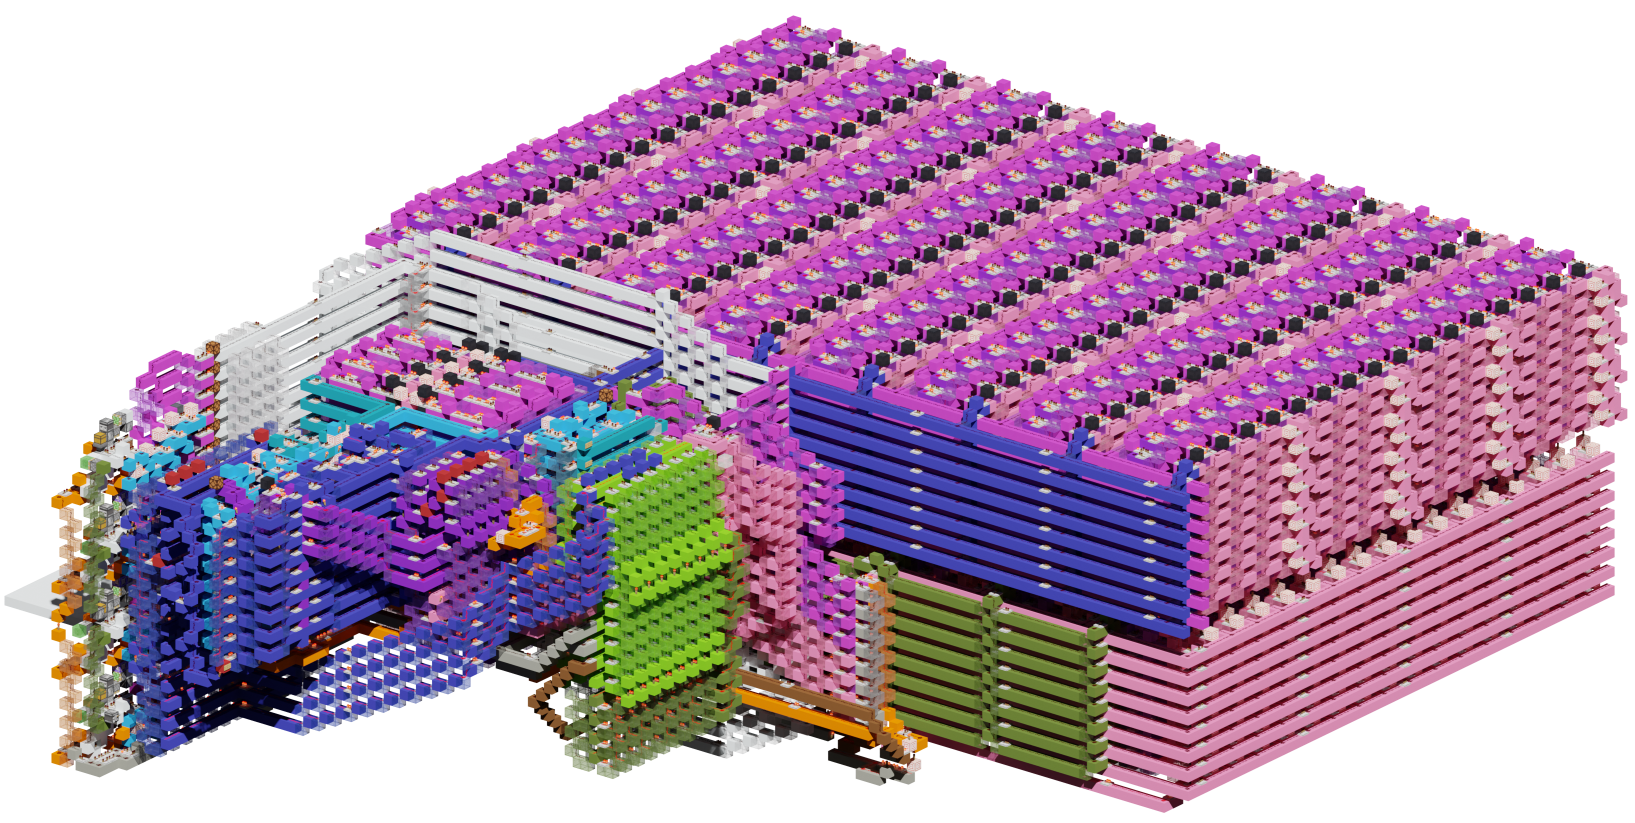
\includegraphics[width=1.1\textwidth]{Figures/CPU-FullShot-small.png}
	\end{center}
\end{figure}

\vspace*{.02\textheight}

\vspace{1.5cm}
\large \textit{A thesis submitted in fulfillment of the requirements\\ for the degree of \degreename}\\[0.3cm] % University requirement text
% \textit{in the}\\[0.4cm]
% \deptname\\[2cm] % Department name
\vspace{0.5cm}
%\vfill

{\large \today}\\[4cm] % Date
 
\vfill
\end{center}
\end{titlepage}



%----------------------------------------------------------------------------------------
%	ABSTRACT PAGE
%----------------------------------------------------------------------------------------

\begin{abstract}
	\addchaptertocentry{\abstractname} % Add the abstract to the table of contents
	This project aims to create and explore the design of a basic 8-bit CPU using concepts and ideas acquired over years of interest in the subject as well as some direct research into the inner workings of the core of all the machines we use on a daily basis. While the background concepts of CPU architecture were learned from valuable sources, most of the implementation stems from trial and error and ideas thought up by myself, which, as will be discussed in the final chapter, led to some avoidable difficulties and limitations in the potential of the CPU. Nevertheless, the CPU is capable of solving basic arithmetic and logical expressions and, with 256 bytes, has the potential to run some slightly more complex programs, even including some fixed-point arithmetic. The main goal of this project was to understand what goes on at a very low level, equivalent to the transistor level in real CPUs, and laying the foundations to make bigger and better CPUs in the future. This goal was, in my opinion, definitely achieved.
	\end{abstract}


%----------------------------------------------------------------------------------------
%	ACKNOWLEDGEMENTS
%----------------------------------------------------------------------------------------

\begin{acknowledgements}
	\addchaptertocentry{\acknowledgementname} % Add the acknowledgements to the table of contents
	Firstly, I would like to thank my supervisor, Dr. Thomas Preu, for his critical but ever constructive aid, as well as giving pointers where they were needed and keeping me on the right path when I tended to veer off it. I give many thanks and much love to my parents, who always showed interest in what I was working on and gave their personal insights. Finally, I want to thank my good friends who were often present and made for pleasant, fun company throughout the year.
	\end{acknowledgements}
	

%----------------------------------------------------------------------------------------
%	LIST OF CONTENTS/FIGURES/TABLES PAGES
%----------------------------------------------------------------------------------------

\tableofcontents % Prints the main table of contents


\chapter{Foreword}

\label{Foreword}

Minecraft is one of, if not the most popular modern game on the market. Loved and known by millions of people, it offers the player a vast, near endless world and the creative freedom to build whatever their imagination allows. The game continues to add new features and blocks to its inventory, allowing for ever-expanding horizons of potential for each one of the players. The vast possibilities of gameplay allow for many play-styles to occur. There are the standard survival players that play the game by the game's rules, slowly building up their base and building small farms, exactly as the creators of the game intended. Then there are the builders, the artists of Minecraft, who express their creativity within the scope of the game and its array of blocks and construct awe-inspiring builds on every scale, from small houses with incredible detail in their design to cities, castles or statues that scratch the ceiling of the world. There are the players that add their own modifications on to the foundation that Minecraft provides, to the extent that it almost seems like another game entirely. Each player can choose what they want to do, and is never confined to just one category, since there are usually no clear lines distinguishing one play-style from another.

Myself, I chose to explore the area of computational redstone, after being blown away by the things that the community has created. Seeing actual computers and calculators in this incredible game left their mark in me, and while the builders of Minecraft seemed just as alluring, computational redstone was more intriguing. With some experience in basic programming and having created some very simple games that, admittedly, are not worthy of mention here, my interests began wandering deeper into the functionality of the computers we interact with almost every moment of our waking lives. As with most subjects nowadays, this one was best explored online, specifically YouTube, where there is an enormous amount of information regarding computer science and computational logic. I'd like to point out two people in particular who have by far taught me the most in this subject. Ben Eater \cite{BenEater} had previously worked at Khan Academy, one of the best online learning sources. Eater creates educational YouTube videos on all things regarding the inner workings of computers and procedures on the lowest levels, working on breadboards to create his own circuits. His most impressive series is the 8-bit CPU on a breadboard, where he goes into the details of why and how everything he makes is needed and works, and which served as the main inspiration for this thesis. The other person is Mattbatwings, another educational video creator, is a computer science student who focuses on teaching computational logic in Minecraft to a broad audience. He laid the foundations for many concepts and circuits which I've modified and built upon in creating my CPU.

Mods, or modifications, are a big part in designing larger creations, both in the realm of redstone or that of builders. The big one is \textit{World Edit}, allows for copying and pasting volumes, or stacking volumes in a series of itself, a feature that, when looking at the RAM, the big chunk of memory behind the CPU, can quickly be justified for its use. This mod is an incredible time saver, allowing for rather quick iteration, without which designing this CPU within the span of a year would have been practically impossible. The other mod, which came into play for debugging and executing programs is the \textit{Carpet} mod for its time-control features, where the speed of the game can be modified from 20x slower up to 50x faster.

Designing the CPU was largely a case of trial and error. The knowledge gained over the past few years served almost entirely as a foundation upon which the layout, architecture and interaction between each component were designed. Initially a prototype was made to better understand the relationships between each part of the CPU and how the instructions could work. Many things changed between the prototype and the final design, improving the connections to be more efficient, but also carrying over some design flaws and inefficiencies, which will be discussed later on.

\mainmatter % Begin numeric (1,2,3...) page numbering

\pagestyle{thesis} % Return the page headers back to the "thesis" style

\chapter{Building Blocks of Logic} % Main chapter title

\label{Chapter1}

%-----------------------------------
%	section Classic Electrical Circuits
%-----------------------------------

\section{Classic Electrical Circuits}

\subsection{Signal Transmission}
Signal transmission in electronic circuits has a few major differences to that in the redstone circuits of Minecraft. First, most signals in the electric connections are bidirectional, while Minecraft, due to needing to use repeaters every few blocks, can only send signals in one direction. Secondly, Minecraft has no concept of closing a loop or shorting a circuit or anything related to voltage or amperage. Third, and most significantly, the speed difference of transmissions in the two subject matters are hard to imagine. The electromagnetic wave ripples through the wire at around 90 percent the speed of light, depending on the physical characteristics of the wire, which is ca. 2.7 * 10$^8$ m/s. The equivalent signal in Minecraft will travel at most at 18 blocks per RT, unless some unintended game mechanics are used, or 90 blocks per second in optimal conditions. A real CPU is around 4cm x 4cm in Area, while the CPU in this project takes up around 100 x 100 blocks, give or take. A signal can thus go from one side of the CPU to the opposite in 0.14 nanoseconds, or 1.4 * 10$^{-10}$s in a real CPU, whereas the Minecraft equivalent takes about 1.1s. Not even considering the increased complexity of the actual CPU, where a simpler one could be made significantly smaller, this equates to a speed ratio of 1 to 6.75 billion, or 9 orders of magnitude.

\subsection{Clock and Instruction Cycles}

In the x86 Instruction Set, a single instruction execution can cost from one up to dozens - and in rare cases, over a hundred - clock cycles. Take, for example, the Intel Pentium P5 processor \cite[Page 162 - Intel Pentium]{InstrTable_Agner}, a 32-bit processor running its clock at speeds from 60MHz up to 300 MHz. Its simplest operations, such as moving data from memory to register (MOV), can be executed in a single clock cycle, or simple logic operations, like adding a number from memory to a number from a register (ADD), takes only two clock cycles. Most operations, however, will take multiple clock cycles, though usually less than ten. An integer division (IDIV), however, the most expensive non-floating-point operation on the Pentium P5, will cost 46 clock cycles for two 32-bit longs. Some floating point operations are even more expensive, such as the floating point arctangent of a value (FPATAN) at a cost of 120-146 clock cycles. The reason for these high amounts of clock cycles is that some specific hardware components, like an integer division component, work in internal loops or on long conveyor belt type operations, and the instruction needs to wait until the entire operation is completed before it can access the computed result.

In some cases, mainly the conveyor belt type operations, the instructions can be pipelined, as they are often in actual conveyor belts, and the results can be spit out at a much higher frequency, but the delay between input and the corresponding output stays the same. In that case, the operation can be thought of as a classic Ford car manufacturing factory, where a car gets finished every few minutes or hours, but still may take days or weeks to make it through the entire system.

The reason for why even most of the simple instructions take multiple clock cycles is because of the complexity of the processor not allowing for direct connections between most components. The only method of communication between the major components that perform the logic is via the central data bus, and that can or should only be written to by one component at once. Thus, the instructions are split up into multiple cycles, so each piece of information can get through the processor to its destination.

The way the components are connected together in this CPU is not as simple as a single data bus, but where each component receives its input from all its sources directly and, by carefully setting the control bits, managing to never have any two sources arrive at the same destination and overwriting each other. While this does make the implementation of some instructions significantly harder and increasing the complexity in that regard, the benefits are much faster execution of instructions. This does limit the usage of slower hardware integrated circuits such as a multiplication or division, which thus need to be done in software. Adding any such hardware would drastically increase the complexity of the CPU and its instruction cycle. It is certainly in the scope of a Minecraft CPU, but not in the scope of this project. Thus, the slightly complex but easier to handle version of one clock cycle per instruction is the direction chosen for this CPU.

%-----------------------------------
%	section Minecraft Circuits
%-----------------------------------

\section{Minecraft Circuits} \label{ssec::MinecraftCircuits}

\subsection{Redstone Fundamentals}
Redstone, in its most basic form, is a wire that can be either on or off. If it is on, it holds a certain signal strength, between 0 and 15, which decreases by one each block. Through the redstone wire, it travels instantly, but once the signal strength reaches 0, it stops. Therefore, the signal needs to be renewed, at the cost of adding some delay. Whereas the game physics run on 20 ticks per second, i.e. the state of each block gets updated 20 times a second, the delays from redstone components take 2 ticks, or 1 redstone tick (RT), or a multiple of that. It is therefore common to refer to timings in redstone in RT. The fixed limit of 20 ticks per second can be modified using third-party mods, which can set the limit up to 500 ticks per second, though at that point the game usually cannot update itself fast enough to reach that limit.

\begin{figure}[!ht]
    \begin{center}
        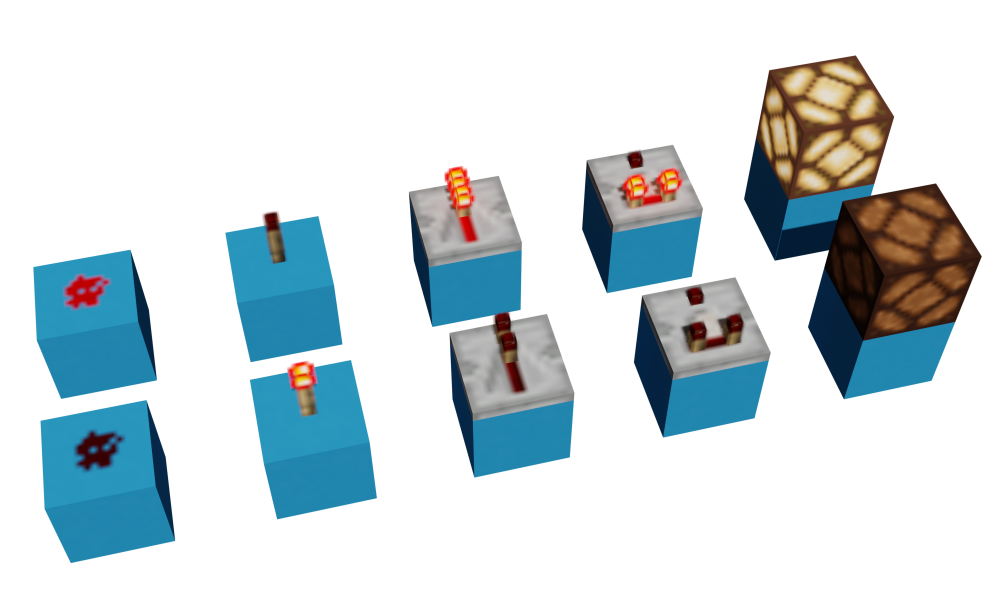
\includegraphics[width=0.7\textwidth]{Figures/Components-small.png}
        \caption[Five basic components]{From left to right: Redstone Dust, Redstone Torch, Repeater, Comparator and Redstone Lamp}
        \label{fig::RedstoneComponents}
    \end{center}
\end{figure}

\subsection{The Components} \label{ssec::Components}
There are five main components to redstone circuits: Redstone dust, the redstone torch, the repeater, the comparator and the redstone lamp as shown in Figure \ref{fig::RedstoneComponents}. The redstone torch will, in its normal state, emit a signal at full power to surrounding blocks, while powering the block above it in a way that the signal goes through the block and powers the surrounding blocks. If the block the redstone torch is connected to is powered, the redstone torch turns off, a property that is most commonly used as an inverter or a NOT gate.

The repeater, when powered from behind, emits a signal at full power into the block it is facing into, much like the redstone torch powers the block above it. The repeater can also be locked when powered from its side by another repeater. In the locked state, the repeater holds the power state it was in when it got locked and ignores any changes to its input, effectively storing one bit of data. The repeater can be manually configured to a specified delay between input and output within a range of 1-4RT, giving the user fine control over the time a transmission takes, something that is nearly impossible (and usually not wanted) in electronic circuits.

The comparator is possibly the most misunderstood redstone component by the playerbase, referring to its two modes and their interaction with signal strengths. The normal use case is to read out the signal strength from its input or the fill-level of the container behind it, where the fill-level is represented by a signal strength, and emit that signal strength in the front. Comparators can also receive inputs from the side, which interact differently depending on which mode the comparator is set to. In comparison mode, the comparator works as follows: If the signal from the main input is stronger than the signal from the side, it will output its received signal as it gets it, otherwise it doesn't emit a signal. In subtract mode, the comparator always subtracts the side input from the main output. This functionality allows it to be used a simple binary switch to control the flow of a signal. A common use case for the comparator in this CPU is as a pulse-width limiter, as shown in Figure \ref{fig::ExampleCircuits} on the right. When the circuit receives a signal, it first goes unhindered through the comparator with the standard 1RT delay, while the signal also passes through the repeater on the side, set to some delay. After the delay specified by the repeater, the signal is input on the side of the comparator at full strength, blocking any further transmission. This way, the maximum length of a signal going through the circuit is that specified by the repeater.

\subsection{Example Circuits} \label{ssec::ExampleCircuits}
Figure \ref{fig::ExampleCircuits} shows three important circuits. The first circuit is the classic AND gate nearly any redstone user in Minecraft will be familiar with. The two inputs control the redstone torches on the blocks, which act like inverters or NOT gates, i.e. an ON signal turns them off. As long as at least one torch emits a signal, the torch in the middle lane remains off and the output is off. Only when both inputs are on will the redstone dust in the middle unpower and allow the center torch to turn on again. The second circuit is the most commonly used XOR gate due to its simplicity, though it is pretty big. The comparators are set to subtract mode, so it will always output the main input minus the input from the side. This gate makes use of the fact that a signal loses strength over distance to check whether only one input is on. If only one input is on, the XOR gate outputs a signal. The best way to understand this gate is to simulate its function by manually counting the signal strengths at each comparator input. The last one is the aforementioned pulse limiter, as described in Section \ref{ssec::Components}, set to a pulse width of 3RT.

\begin{figure}[h]
    \begin{center}
        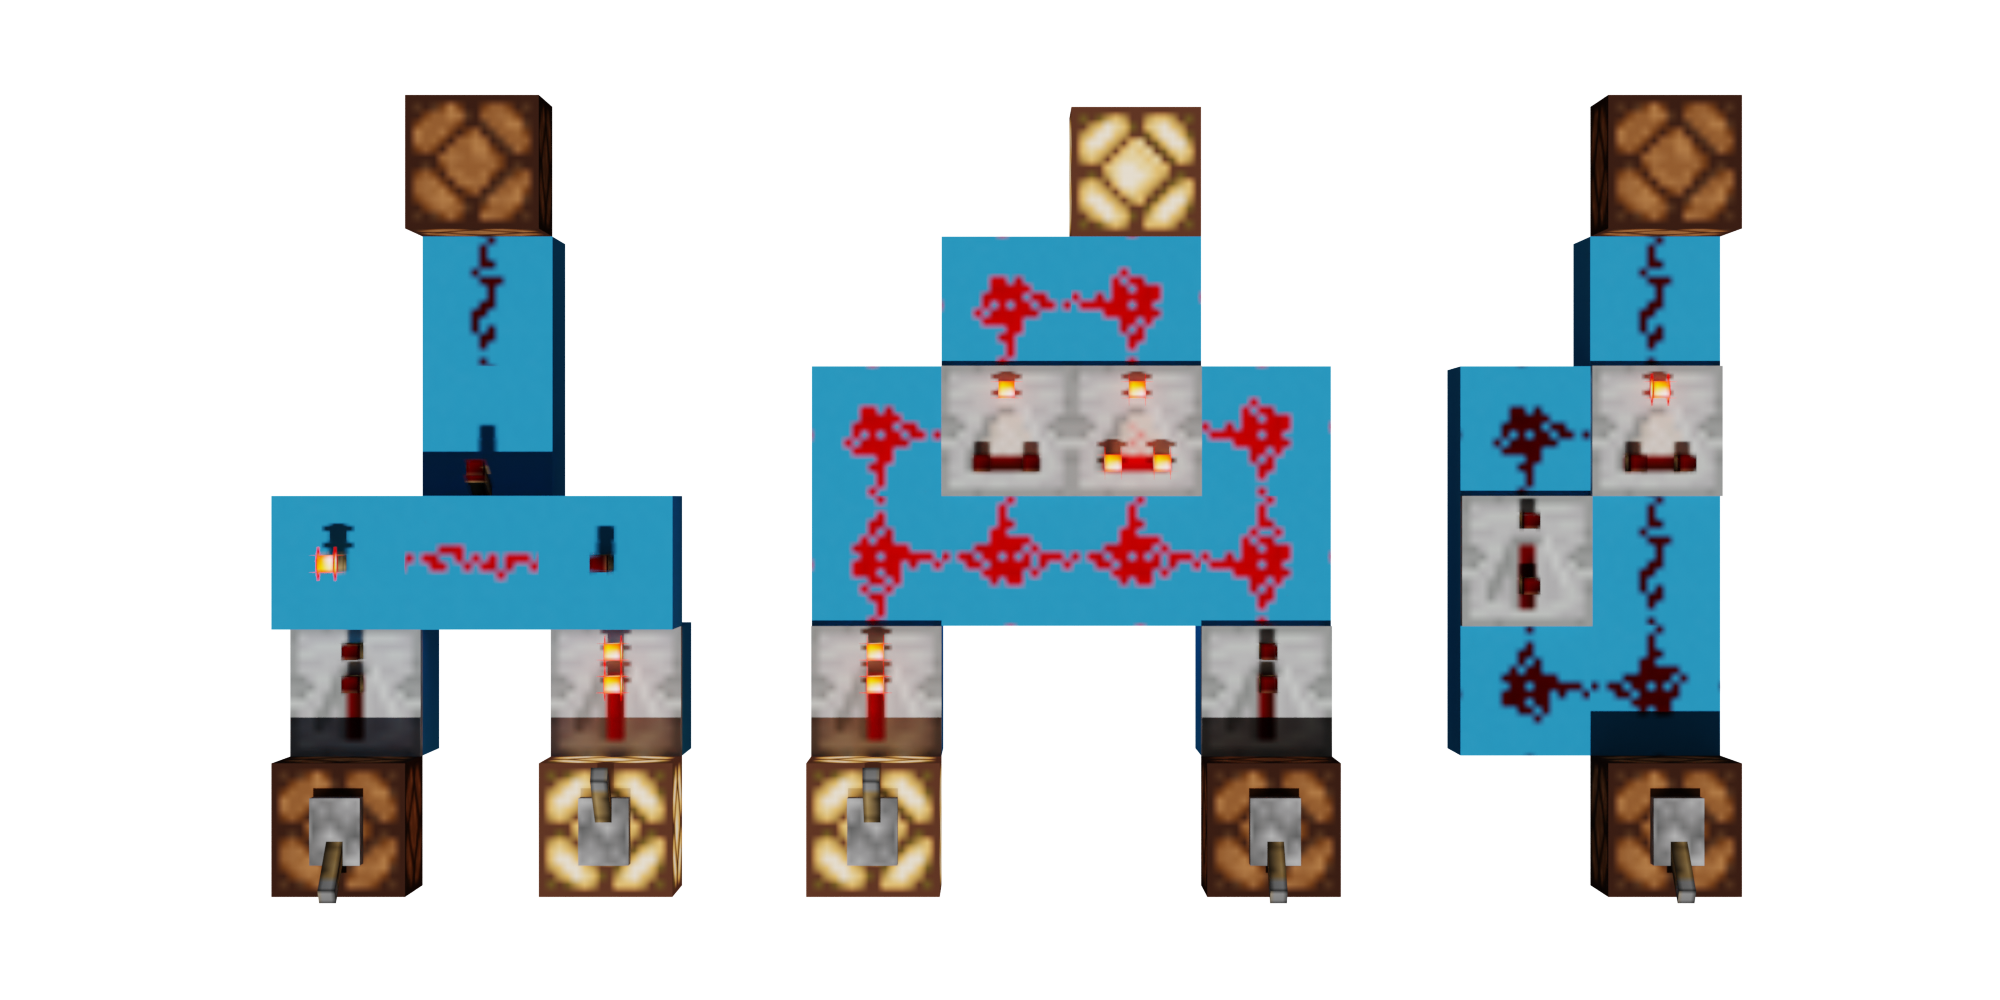
\includegraphics[width=0.9\textwidth]{Figures/ExampleCircuits.png}
        \caption{AND-Gate, XOR-Gate, Pulse-Width Limiter}
        \label{fig::ExampleCircuits}
    \end{center}
\end{figure}


\chapter{Design}

\label{Chapter2}

\begin{figure}[!h]
    \begin{center}
        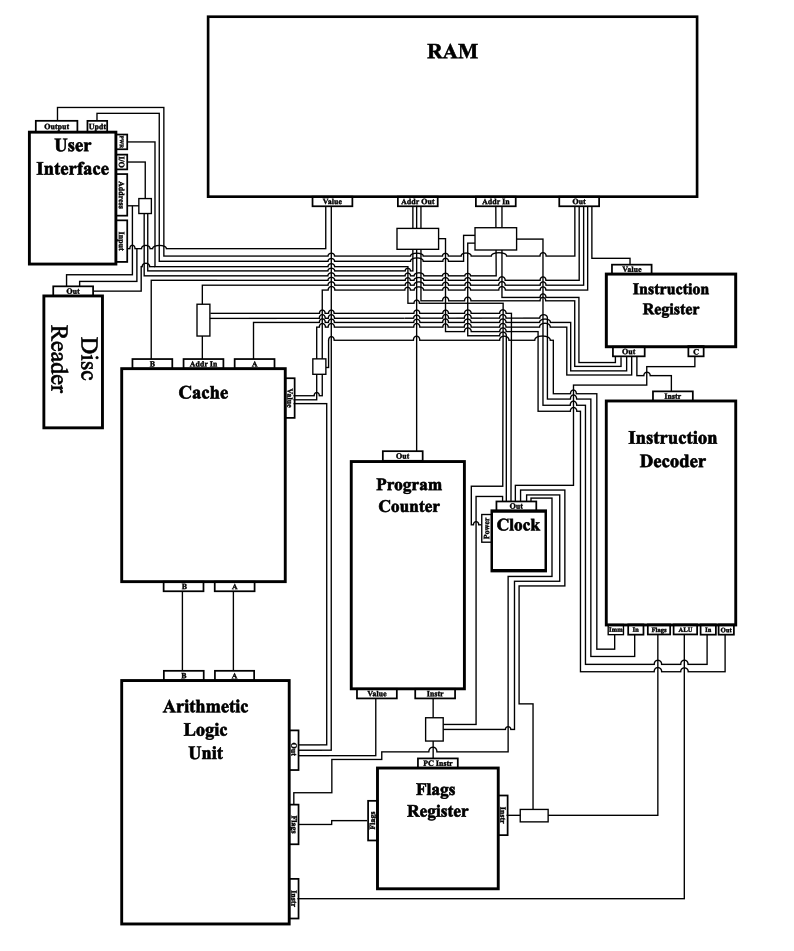
\includegraphics[width=0.49\textwidth]{Figures/Layout_1.png}
        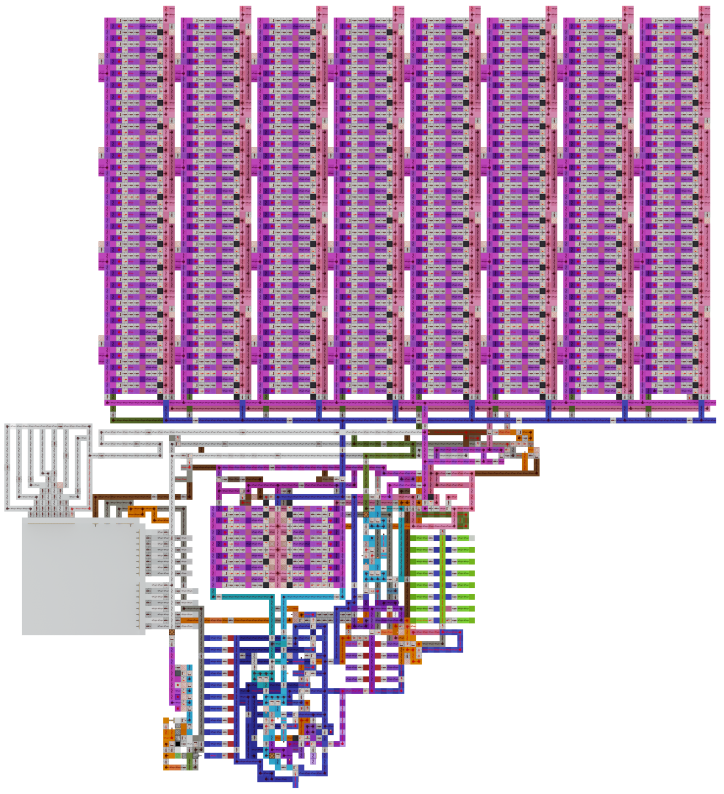
\includegraphics[width=0.49\textwidth]{Figures/CPU-Full-small.png}
        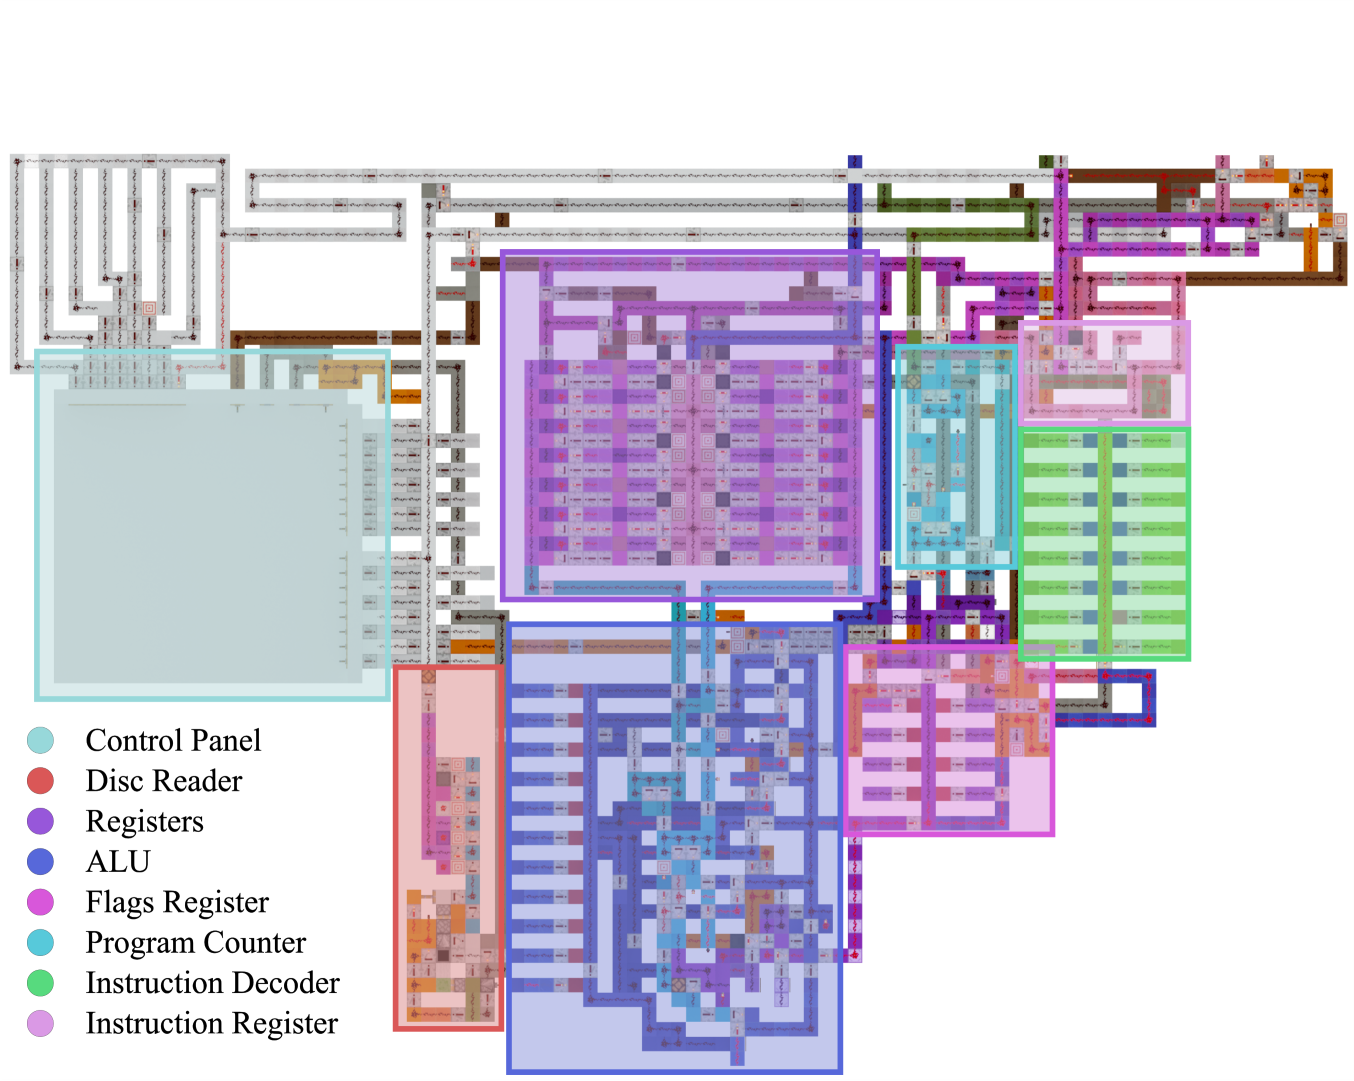
\includegraphics[width=0.8\textwidth]{Figures/CPU-Core-small.png}
        \caption{Placeholder overview of the CPU}
        \label{fig::Overview}
    \end{center}
\end{figure}

\section{Layout and Architecture}
\subsection{Overview}
Figure \ref{fig::Overview} shows three versions of a top-down look on the CPU. The first image is a simplified overview, showing each component in roughly the correct position and scale as well as each line connecting the components, and serves as a reference for exploring the CPU. The image on the right is a top-down render of the entire CPU and its memory to be compared side by side with the simplified overview. The last image shows the CPU without its memory to allow for a better view on the other components which are relative to the memory module much smaller. Each component is highlighted according to the legend next to the image.

\subsection{Architecture} \label{ssec::Architecture}
In chip design, there are two separate architecture principles which dictate the interaction between the CPU and memory. This interaction is often the biggest bottleneck when it comes to how fast the CPU can execute a function. One look at the layout of any CPU and its memory (Figure \ref{fig::Overview} gives an overview over the CPU of this project) will make it clear why this is the case: The memory modules are much larger than the CPU and, while not necessarily very complex, require the CPU to wait for the signal to travel to the furthest memory unit and back to be sure the data has arrived. Even in real chips, where signals propagate at very fast speeds, this is a significant amount of downtime for the CPU. The two architectures tackle the problem in two different ways. The classic and most famous Von Neumann architecture considers all memory to be in the same pool. This means that all memory shares the same address space and is built up the same way, i.e. has the same address and storage size (e.g. 4-bit address and 8-bit storage). Both program data, like variables, and instruction data, like the instruction codes and the arguments, live in the same memory and are accessed over the same data bus. The second option is Harvard architecture, which strictly separates the two pools of memory. All the program data lives in the standard memory space, in RAM, while the instruction data lives in its own space, like a ROM drive or a separate RAM module. The address busses are held separate as well, which allows both the address and the size of the data to be different in each pool. For example, the program data could run on an 8-bit address and use 8-bit data, while the instruction data can have 12bit address space and use 16-bit instructions. Separating the address busses means the CPU can read the instruction and write to memory in the same clock cycle.

Most modern machines will not follow the strict design principles laid out by the two architectures. The line separating instruction and program data is usually blurred in various ways. This is the concept behind modified Harvard architecture. The CPU in this project uses a fairly unique approach to this architecture. It is designed with the Von Neumann architecture at its core, where all program and instruction data shares the same space of memory. There are, however, two separate bus lines, one for the input and one for the output. This allows for similar functionality to the Harvard architecture, where an instruction can be read from and new data written to memory at the same time. The usual advantage of a Harvard architecture based machine being able to have theoretically arbitrarily sized memory units, i.e. each memory unit can have for example an 8-bit or a 24-bit value, independent of what the rest of the computer works on, is mostly lost. This CPU works with instructions of 16-bit lengths, or two memory units, which cannot be accessed at the same time. Therefore, the execution of an instruction happens in two stages. In the first stage, the first byte of the instruction is fetched and stored in the instruction register. In the second stage, the second part of the instruction is output from RAM and is, together with the stored first half, executed. The separate input and output busses as well as the instruction register allow for each instruction to be executed in a single clock cycle, albeit with additional complexity.

\section{Components}

\subsection{Arithmetic Logic Unit}
\subsubsection{Binary Addition}
The ALU is the central part for the purpose of a computer. As the name suggests, the computer's purpose is to compute. Data can be moved and ordered around from one place to another, but without the logical operations and manipulation of data there is no function to the CPU, as none of the data will change, react to or interact with other data. The functions of the ALU are by design very simple, but when combined in bigger sequences allow for highly complex calculations. The functions are addition, subtraction, incrementing, decrementing, binary AND, OR and NOT as well as bit-shift-left and bit-shift-right. The most important functions of the ALU are addition and subtraction. The remaining functions are trivial to implement, requiring one or two logic gates each at most.

\begin{figure}[!h]
    \begin{center}
        \begin{tabular}{@{\qquad} c @{\qquad}| @{\qquad} c@ {\qquad}}
            Base-10  & Base-2 \\
            \hline
            \begin{tabular}{ccc}
                & \tiny{1} & \\
                & 1 & 3 \\
                + &  & 9 \\
                \hline
                & 2 & 2 \\
            \end{tabular}
            & \begin{tabular}{cccccc}
                & & \tiny{1} & & & \tiny{1} \\
                & 0 & 1 & 1 & 0 & 1 \\
                + & 0 & 1 & 0 & 0 & 1 \\
                \hline
                & 1 & 0 & 1 & 1 & 0\\
            \end{tabular} \\
        \end{tabular}
    \end{center}
    \caption{Addition by hand}
    \label{fig::BaseAdditionComparison}
\end{figure}

Addition in a base-2 system, as is the case in binary, works nearly identically to addition in our familiar base-10 system. Starting from the right, the top and bottom digits are added together and the result written to the answer on the same digit. If the result goes over the highest value of a digit, then the next column gets the extra digit carried over. In the normal case of addition, the carry has a value of one and gets added to the other digits in the column (See Figure \ref{fig::BaseAdditionComparison} for an example). To solve the problem of adding multiple-bit numbers, it helps to reduce the problem to adding only two one-bit numbers, in addition to the carry bit. Binary addition simplifies this problem a lot, since each of the three bits can only be in one of two states: 1 or 0. A truth table gives an overview of the expected outcomes when adding a single digit, or two input bits plus the carry bit, as seen in Table \ref{tab::TruthTableOneBitAdder}.
\begin{table}
    \caption{Truth table for single digit addition}
    \label{tab::TruthTableOneBitAdder}
    \begin{center}
            \begin{tabular}{|c|c|c||c|c|}
                \hline C$_{\text{In}}$ & A & B & C$_{\text{Out}}$ & Sum\\ \hline
            0 & 0 & 0 & 0 & 0 \\
            0 & 0 & 1 & 0 & 1 \\
            0 & 1 & 0 & 0 & 1 \\
            0 & 1 & 1 & 1 & 0 \\
            1 & 0 & 0 & 0 & 1 \\
            1 & 0 & 1 & 1 & 0 \\
            1 & 1 & 0 & 1 & 0 \\
            1 & 1 & 1 & 1 & 1 \\\hline
        \end{tabular}
    \end{center}
\end{table}

\subsubsection{Adder Designs}

In classic circuit design, a series of XOR, AND and OR gates is used in a configuration as in Figure \ref{fig::FullAdder}. This circuit fulfills the aforementioned truth table. The output of the sum is then hooked up to the final output and the Carry$_{\text{Out}}$-bit feeds directly into the Carry$_{\text{In}}$ of the next segment, as in Figure \ref{fig::RippleCarryAdder}. This sort of arrangement is known as a ripple-carry adder. The name stems from the fact that the carry bits ripple through from the right to the left side. If every single digit outputs a carry bit, then the carry bit propagates from the right all the way to the left. Since the highest bit does not know if it needs to consider the carry bit, it needs to wait until every previous adder has finished processing its inputs before it can output its sum with confidence that it's correct. The amount of time for the addition to converge to the final answer grows linearly with each additional bit. On modern CPUs that work with 64-bit numbers, this time is not insignificant, but manageable. Alternatives exist that speed up the output, such as carry-skip adders, but the gains are not as significant as the following solution.

\begin{figure}[!h]
    \begin{center}
        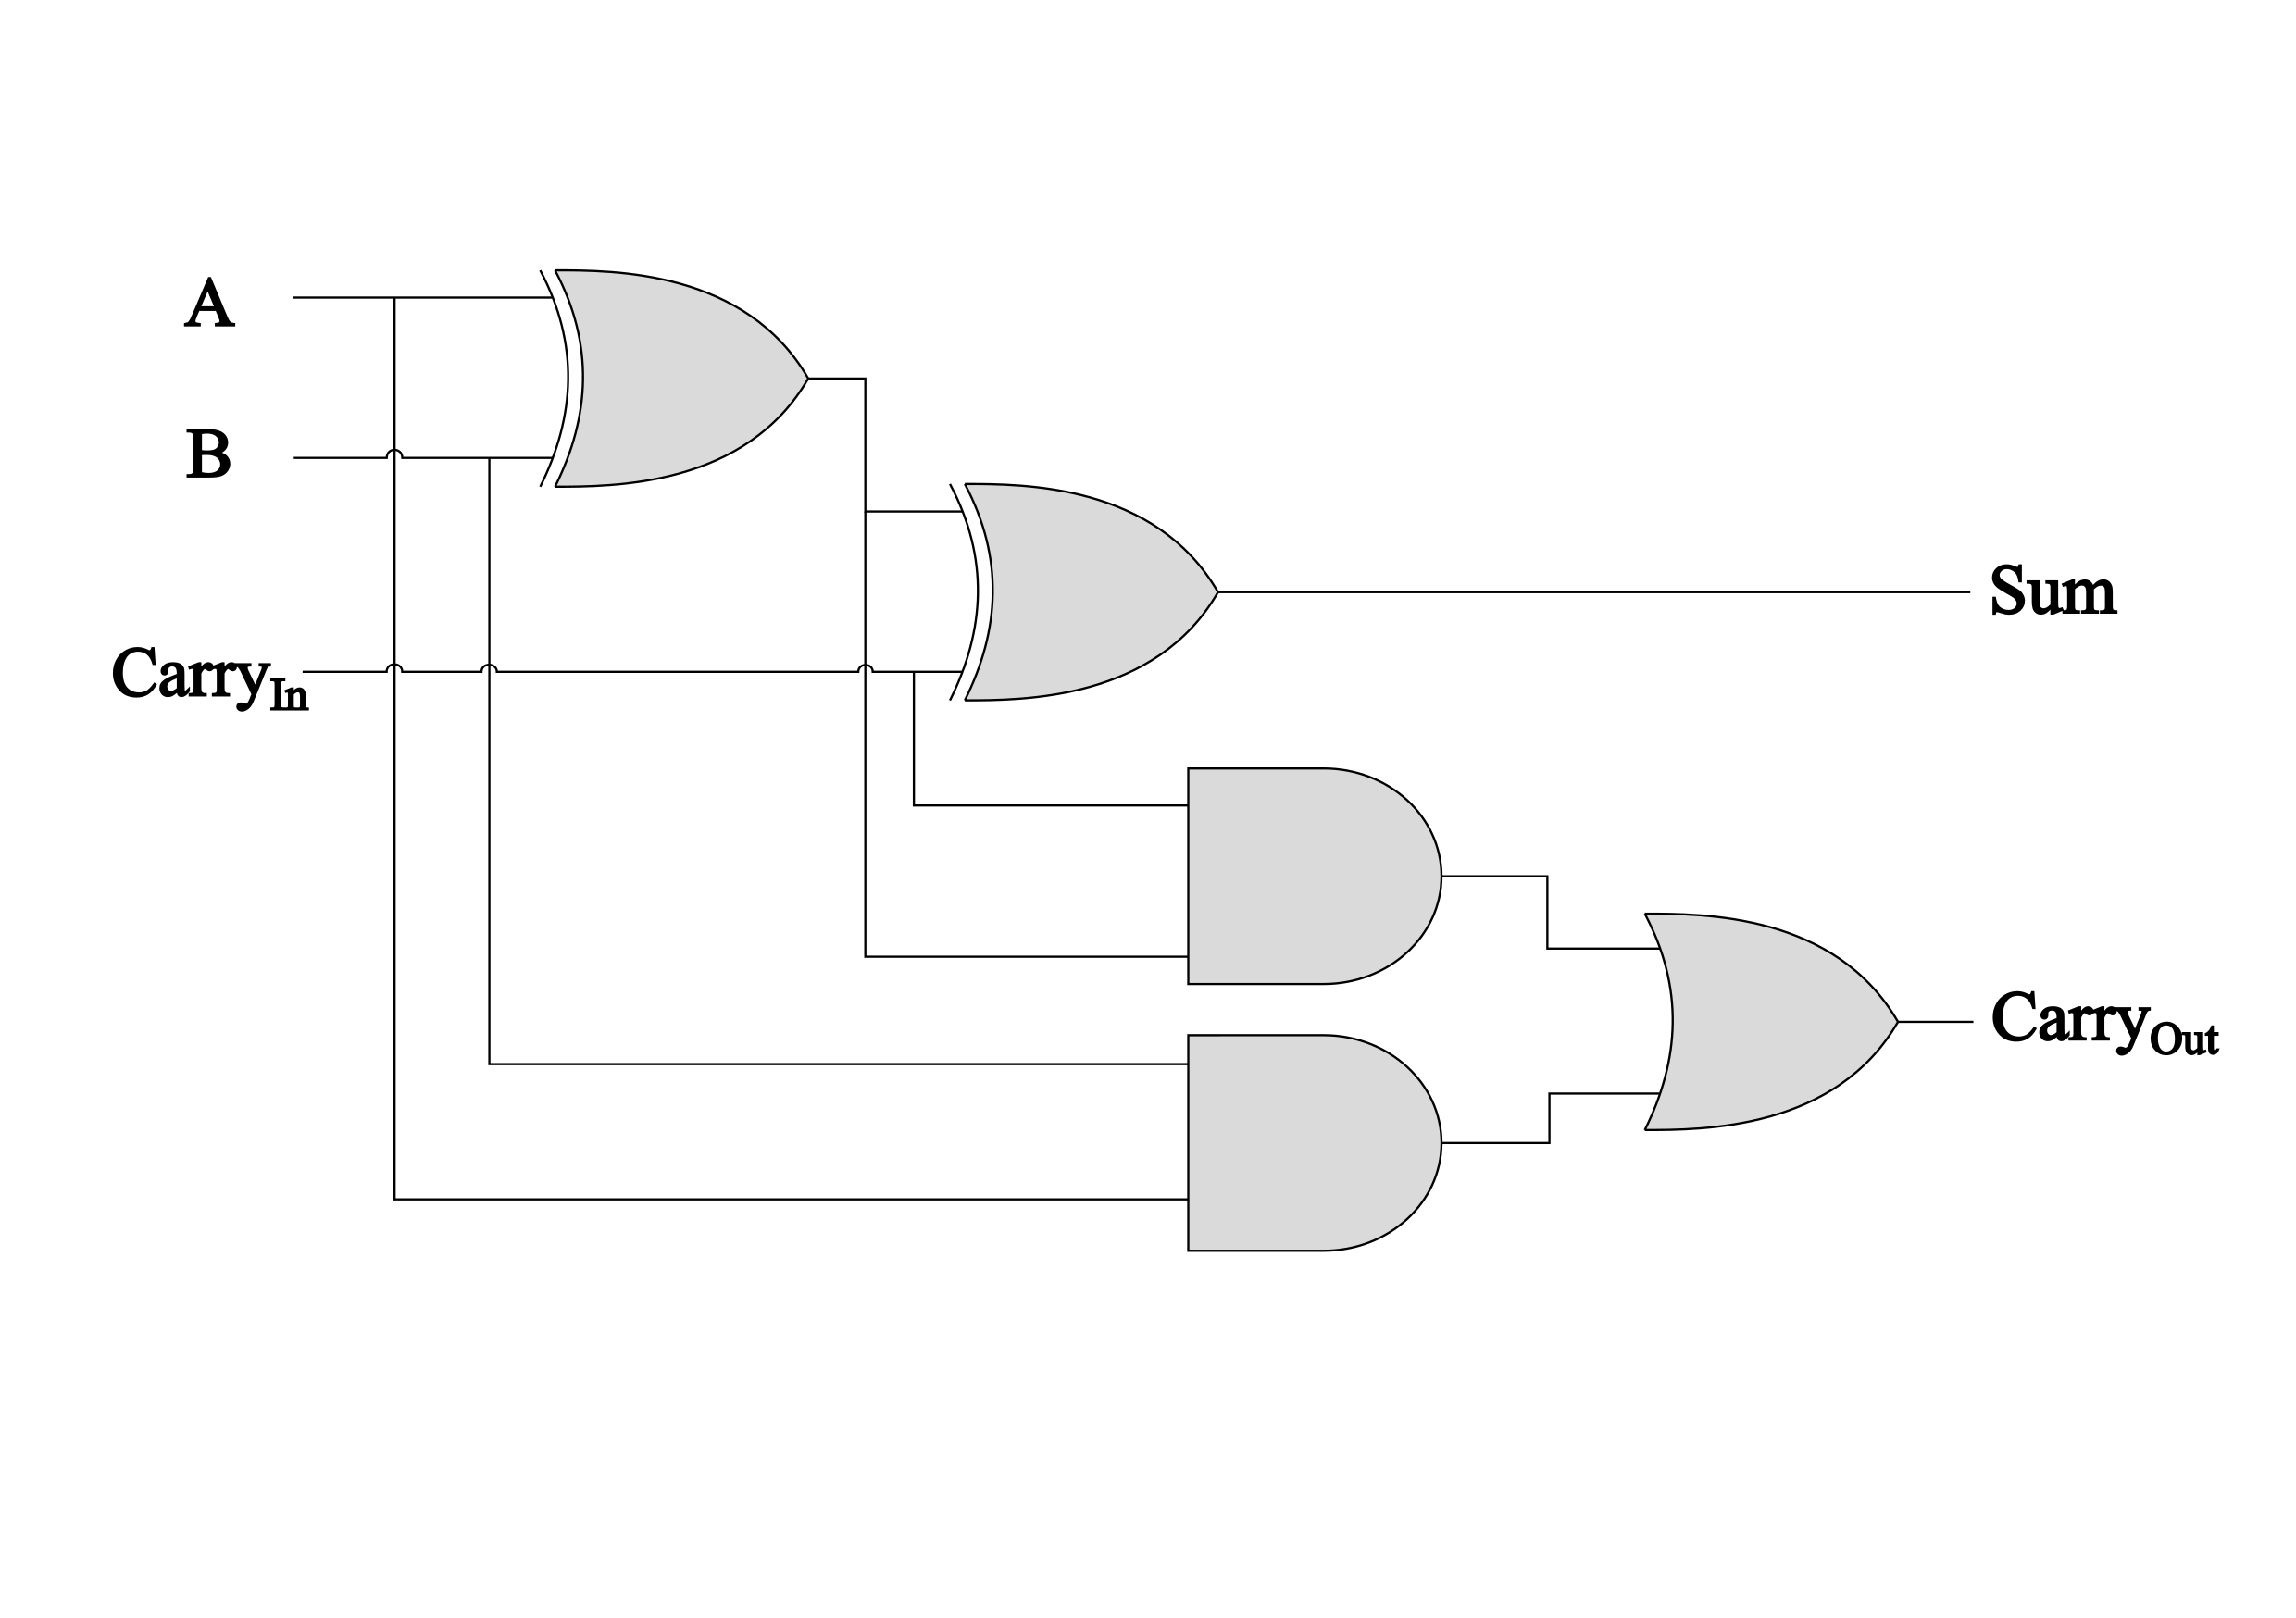
\includegraphics[width=0.48\textwidth]{Figures/FullAdder.png}
        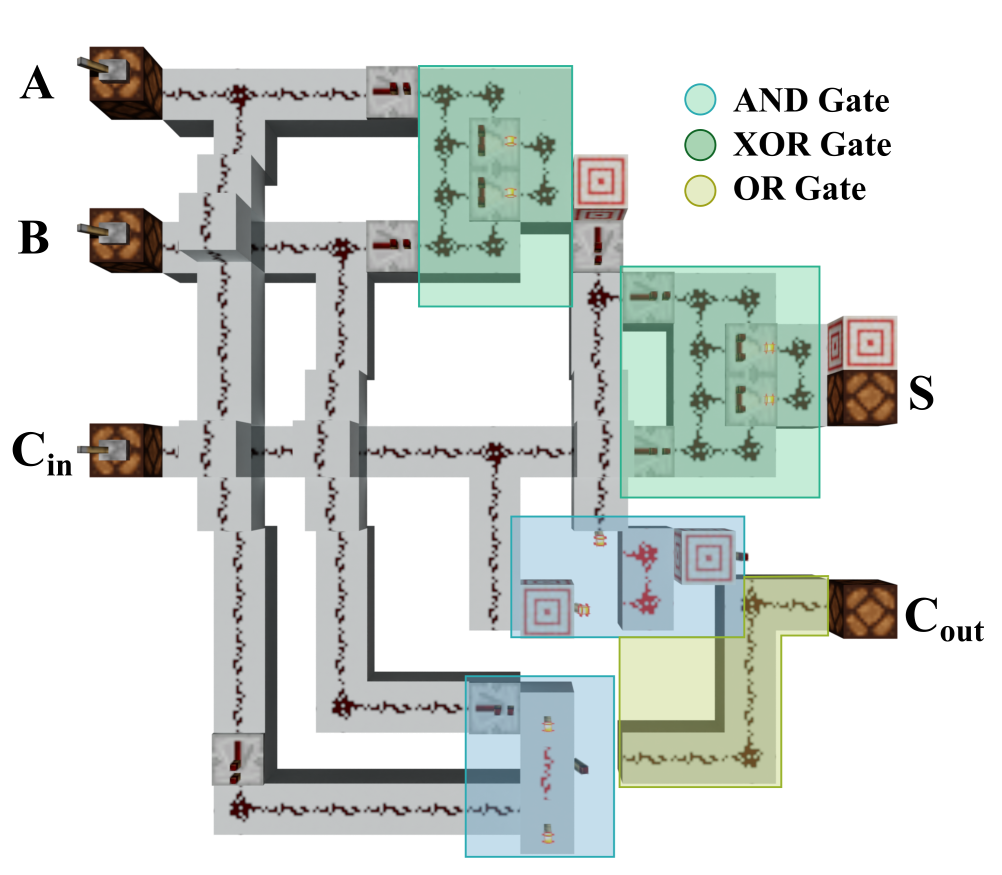
\includegraphics[width=0.45\textwidth]{Figures/FullAdderMC-small.png}
        \caption{One-bit full adder in a diagram and in Minecraft}
        \label{fig::FullAdder}
    \end{center}
\end{figure}

\begin{figure}
    \begin{center}
        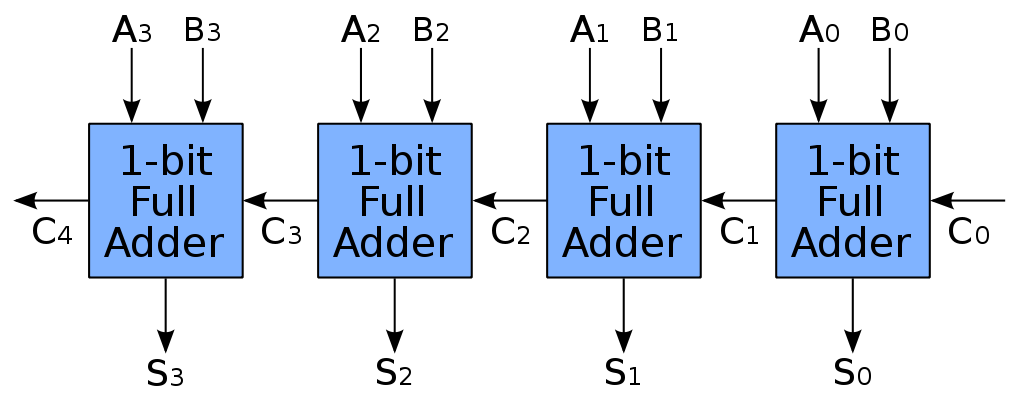
\includegraphics[width=0.6\textwidth]{Figures/RippleCarryAdderWikipedia.png}
        \caption[Ripple-Carry Adder]{Four-bit ripple-carry adder, Source: \cite{RCC_Wiki}}
        \label{fig::RippleCarryAdder}
    \end{center}
\end{figure}

In Minecraft, the time for a single adder to compute its result is around 5RT and each additional carry bit that needs to be processed adds at least 3RT to this time. For a simple 8-bit adder this means a waiting time of 26RT, or 1.3s, until the sum can be read out. This is very inefficient for this project and requires a better alternative. Minecraft's redstone offers a very convenient and simple solution. To improve the speed of the addition, as well as synchronize the outputs, each full adder needs to know beforehand whether it will receive a carry bit or not. Take Figure \ref{fig::AdditionExampleCCA}, where 77 and 75 are added in binary. Notice that the carry operation starts from the first bit, where both bits are 1, all the way to the fourth bit, only stopping when both bits are 0, effectively being cancelled. The only time a carry bit gets generated initially is when both bits are 1, and the only time the carry chain gets stopped is when both bits are 0. This observation is key to optimizing and predicting whether each adder needs an additional carry bit or not. Figure \ref{fig::CCA} shows two layers of the new adder concept, the design of which was mainly taken from the user \textit{Magic} on the \textit{openredstone forums} \cite{CCA_OpenRedstone}. To generate the carry signal (green area with slab ladder), an inverted XOR gate  is used, where it generates a signal when both bits are on or off, and to cancel the carry (red area with slab ladder) a NOR gate is used, only outputting 1 when neither bit is on. The reason why the generate signal is allowed to generate even when both bits are off is because that condition automatically cancels the carry, which takes precedence over the generate signal. These signals are transported up the adder chain, decaying with each block they travel, and then compared at each digit. The stronger signal, i.e. the signal that covers less distance from the right/below takes over, decides whether to add the carry or not. As in Figure \ref{fig::AdditionExampleCCA}, the generate signal at the fifth digit has already lost 4 digits of strength, whereas the cancel signal is newly generated, and will be higher all the way through to the left until a new carry signal is generated. This method works especially well in Minecraft, since the signal strength comparison is an integral part of one of its components, the comparator. A similar implementation in circuit design would probably not grant any benefits, since there is no way to quickly and synchronously compare which signal is stronger or was generated closer.

\begin{figure}[!h]
    \begin{center}
        \begin{tabular}{ccccccccc}
            & \tiny{1} & & & \tiny{1} & \tiny{1} & \tiny{1} & \tiny{1} & \\
            & 0 & 1 & 0 & 0 & 1 & 1 & 0 & 1 \\
            + & 0 & 1 & 0 & 0 & 1 & 0 & 1 & 1 \\
            \hline
            & 1 & 0 & 0 & 1 & 1 & 0 & 0 & 0\\
        \end{tabular}
    \end{center}
    \caption[Carry pattern addition]{Binary Addition showing carry pattern}
    \label{fig::AdditionExampleCCA}
\end{figure}

\begin{figure}[!h]
    \begin{center}
        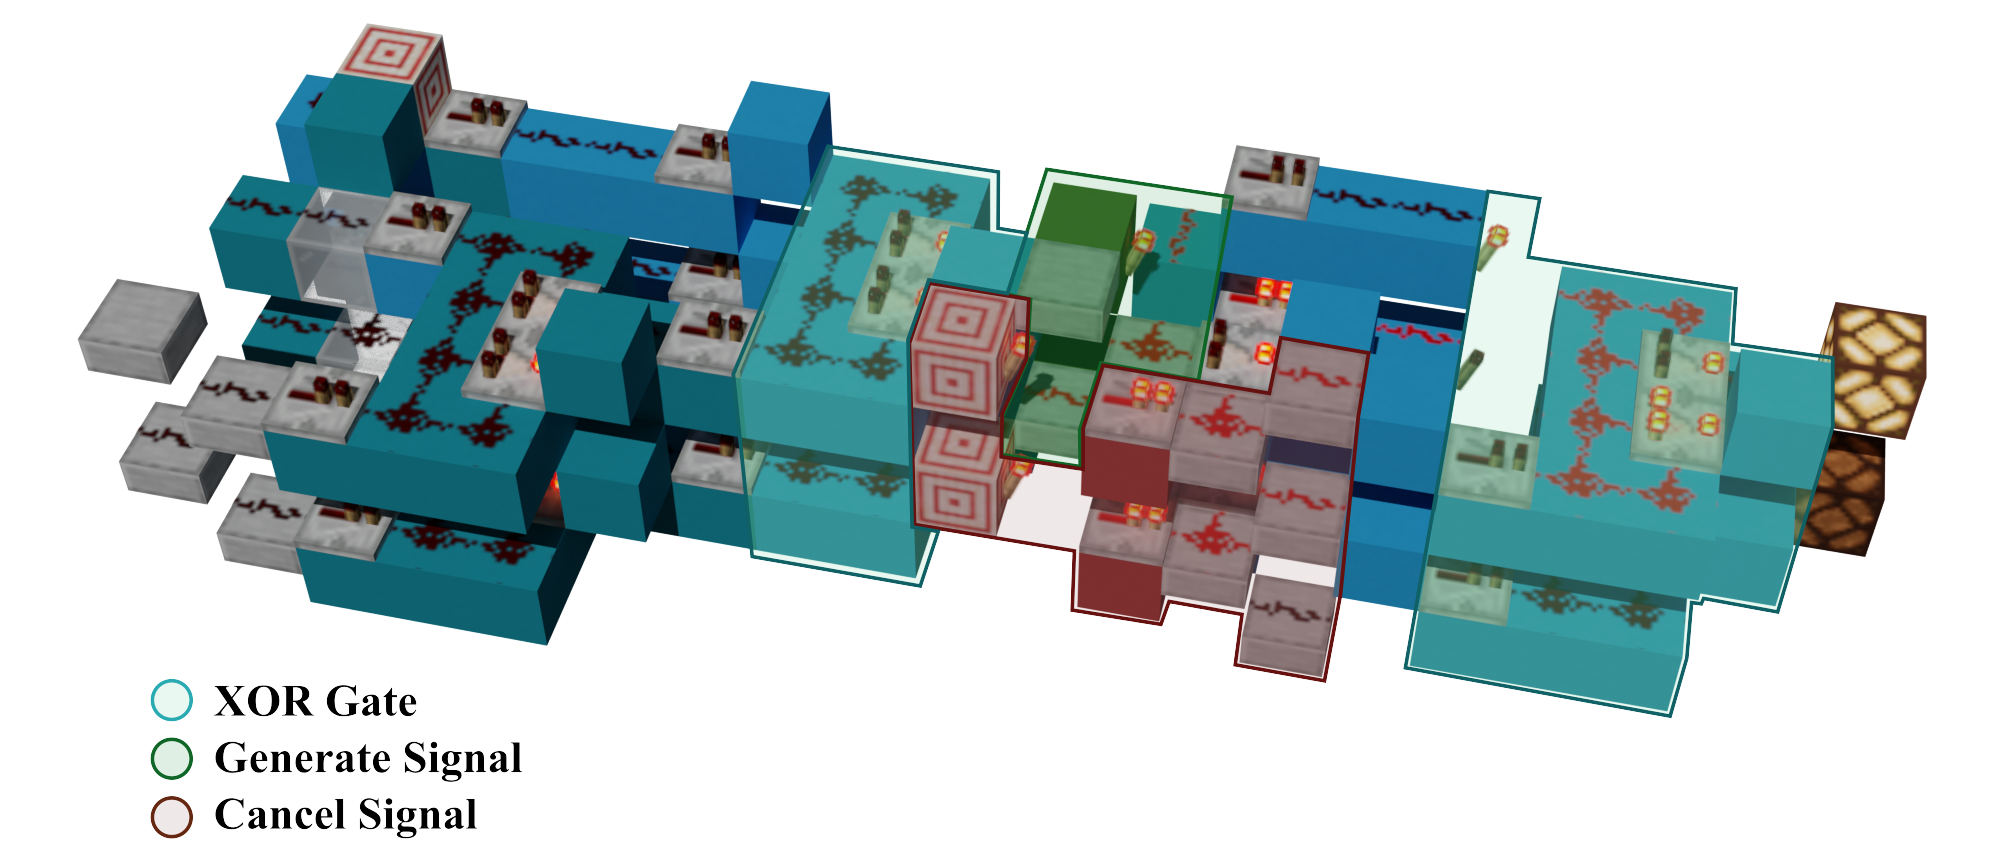
\includegraphics[width=0.7\textwidth]{Figures/CCA.png}
        \caption[Carry Cancel Adder]{Two layers of the Carry Cancel Adder}
        \label{fig::CCA}
    \end{center}
\end{figure}

\subsubsection{Two's Complement}

Currently, the ALU only works with unsigned 8-bit integers, allowing the use of values from 0 to 255. In order to use negative integers, a system to represent negative numbers is needed. The first idea that pops into anyone's mind is to assign the highest bit to the sign bit and say that, if it's 1, the number is negative, and if it's zero, it's positive. Performing simple operations such as binary addition of two numbers now becomes anything but trivial, and would require checks to see if the number is negative before each operation as well as an entirely different truth table to handle the negative numbers, since the corresponding negative analog to the truth table from Table \ref{tab::TruthTableOneBitAdder} would look different. The common standard to use is the so-called \emph{Two's Complement}. This standard assigns the highest bit its own value but with its sign flipped. A 4-bit number in this system would therefore be represented as in Figure \ref{fig::TwosComplement}. To negate a number, all bits are flipped and a one is added. For example, $7 = 0111$ and $-7 = 1001$. Two's complement builds purely on addition, rather than non-linear functions such as the first idea, and only changes the way the number is interpreted, i.e. read by the user. All operations performed on unsigned integers work identically to those from signed integers. The range of an 8-bit signed integer goes from -128 up to and including 127, as can be used in this CPU.

\begin{figure}[!h]
    \begin{center}
        $\begin{tabular}{c|c|c|c}
            \textbf{-8} & \textbf{4} & \textbf{2} & \textbf{1} \\
            \hline
            1 & 0 & 1 & 1\\
        \end{tabular} = 1 * (\textbf{-8}) + 0 * \textbf{4} + 1 * \textbf{2} + 1 * \textbf{1} = -5$
    \end{center}
    \caption[Two's complement example]{Two's complement example of (-5)}
    \label{fig::TwosComplement}
\end{figure}

\subsection{Instruction Unit}
The Instruction Unit's function is the least complex of all the components, its design being identical to a multiplexer, yet its role is as vital as any, as it controls the flow of data through the computer. It takes in a 4-bit instruction code, commonly called the opcode, which gets decoded into a series of control bits, whose purpose is to allow data through specific channels to execute an instruction.

\subsubsection{The Decoder}
The decoder gets its input from the Instruction Register (IR), which always stores the first 8 bytes of the instruction on the first part, the falling edge, of the clock cycle. The IR feeds the opcode, a 4-bit value, into the decoder, which the decoder then uses to turn on or off individual control bits that are connected to each component. Decoding the four bits happens separately in each decoding unit, which are each set to an opcode between 0 and 15. A decoding unit is a NOR gate with four inputs, where each input needs to be off to have an output. Each bit has a preset expected state, where an expected state of 1 gets inverted, so that that input is off when its bit is on, and an expected state of 0 goes through directly, so when that bit is off, that input is also off. If each bit corresponds to its expected state, all the OFF-bits will continue to be off and all the ON-bits will be inverted into an off state, resulting in the output line being off (see Figure \ref{fig::MemUnit}). The output line can now be used to turn on whichever control bits it requires to be turned on by sending the redstone signal through to the control bit. In the component, the control bits that are meant to be on for each opcode have a red block on their corresponding line to allow the signal to pass through them.

\subsubsection{Control Bits}
The Instruction Unit controls the four main channels of the CPU. The STR control bit enables the output of the Registers and sets the write-line of the RAM high, so that, when the clock goes high, the data is written into RAM. That control bit is only used by one instruction but is necessary for the CPU to write program data, like variables, into memory. The IMM and IN control bits control the inputs to the Registers. The IMM bit specifies that the input to the Registers is an immediate from the instruction data, an 8-bit integer from RAM rather than an output from the ALU. The IN bit is used to tell the Registers to store the available data once the clock goes high. The next three bits labeled PC 1 through 3 send an instruction code to the program counter, where it's processed further to determine whether a jump or a simple increment should occur. Finally, the ALU control bits send another instruction code to the ALU, where the instruction decodes again into a single ALU operation.

\subsection{Read Write Addressable Memory}
While executing a program, the CPU needs to keep track of various variables as well as modifying or computing new values. The Random Access Memory (RAM) and the Registers are used to store and output data on command. The RAM unit is a big array of registers that each have an 8-bit address and 8 bits of data. The Registers module in the CPU consists of 14 read-write registers that are connected directly to the ALU and the PC. They play the middleman in any operation of the CPU. Any time an instruction is executed, at least one register is specified which contains a value for the execution of the instruction. The jump instruction, for example, takes a register address as an argument to which to set the program counter to: JMP 0r3 sets the program counter to the value of whatever is in register at address 3.

\begin{figure}[bp!]
    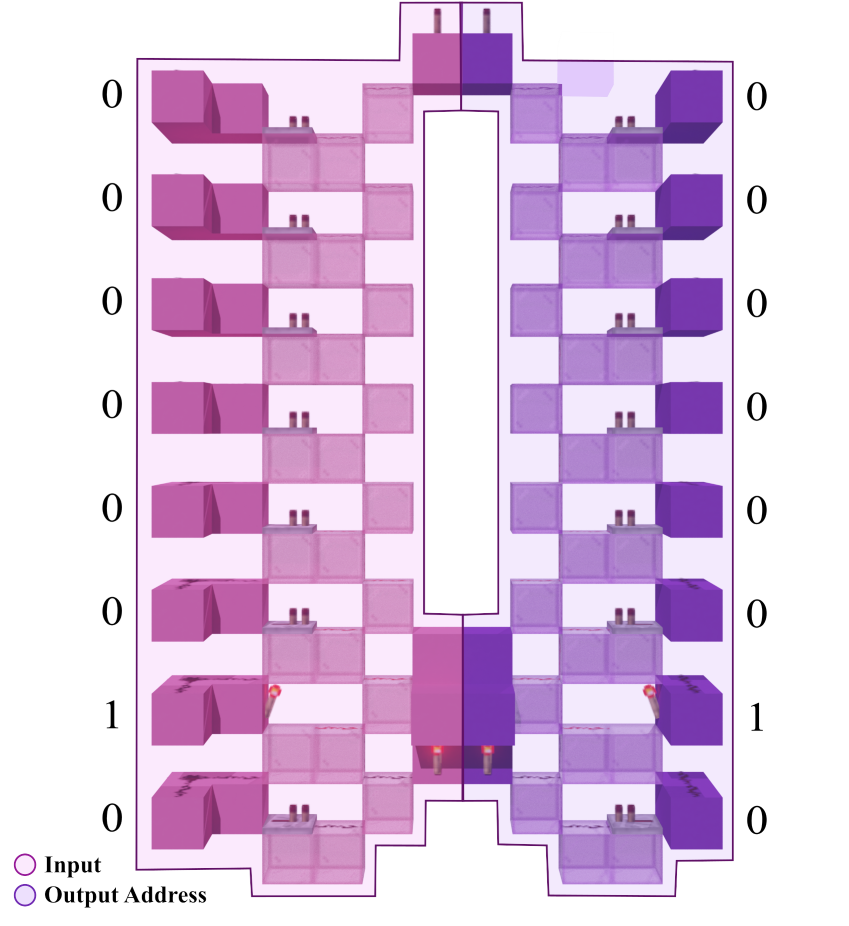
\includegraphics[width=0.48\textwidth]{Figures/MemUnit-small.png}
    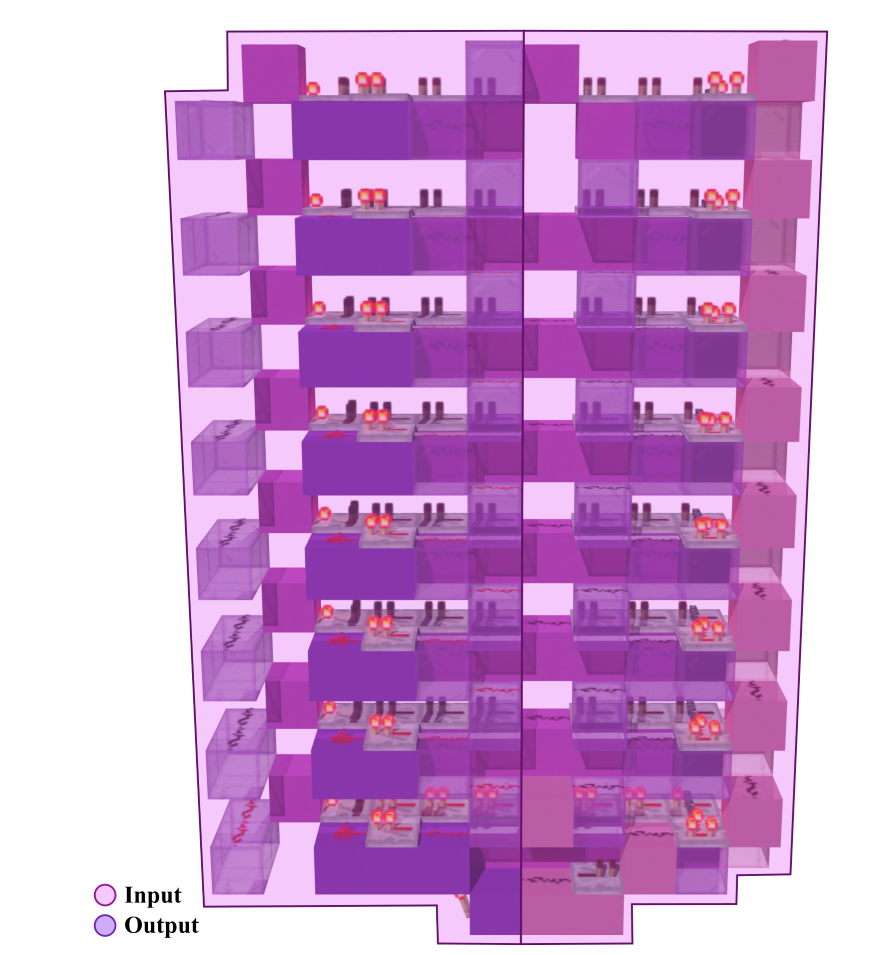
\includegraphics[width=0.48\textwidth]{Figures/MemUnit_1-small.png}
    \caption[Register Module]{Register with an address of 2, or 0b00000010 (displayed in the graphic). The decoder on the left, the memory unit on the right}
    \label{fig::MemUnit}
\end{figure}

The Register is built up of a decoding unit and a memory unit. Figure \ref{fig::MemUnit} displays the decoder on the left, set up for address 2, and the memory unit that sits above it on the right. The decoder is the same as the one from the Instruction Decoder, where each register gets an address. In the case of the RAM, the address is incrementally set from 0 to 255, using up the full range of eight bits, whereas the registers only go from address 1 to 14. The memory unit uses lockable repeaters to store data. By quickly unlocking and re-locking a repeater, the repeater gets set to the state of the redstone behind it from the data line. This sequence starts as soon as the decoding unit receives the correct address. The clock, along with the control bits from the instruction decoder, controls when the address is allowed to go to the decoding units and the subsequent writing of data.

\subsection{Program Counter}
The purpose of the program counter (PC) is keeping track of what line of the program the CPU is currently executing. In essence, it is a pointer to the RAM module as the read address and is the only way for data to be read from RAM. The PC counts up each clock cycle to the next instruction, which is typically two bytes further than the current instruction. Each instruction is two bytes long and thus is stored in two separate registers in RAM. After the first byte of the instruction has been fetched and stored on the falling edge of the clock, the PC will always increment once to fetch the second half of the instruction. On the rising edge of the clock, the program counter's next action depends on the instruction, which can either increment the PC or give it a jump command, referred to as a branch in the program.

\begin{figure}[bp!]
    \begin{center}
        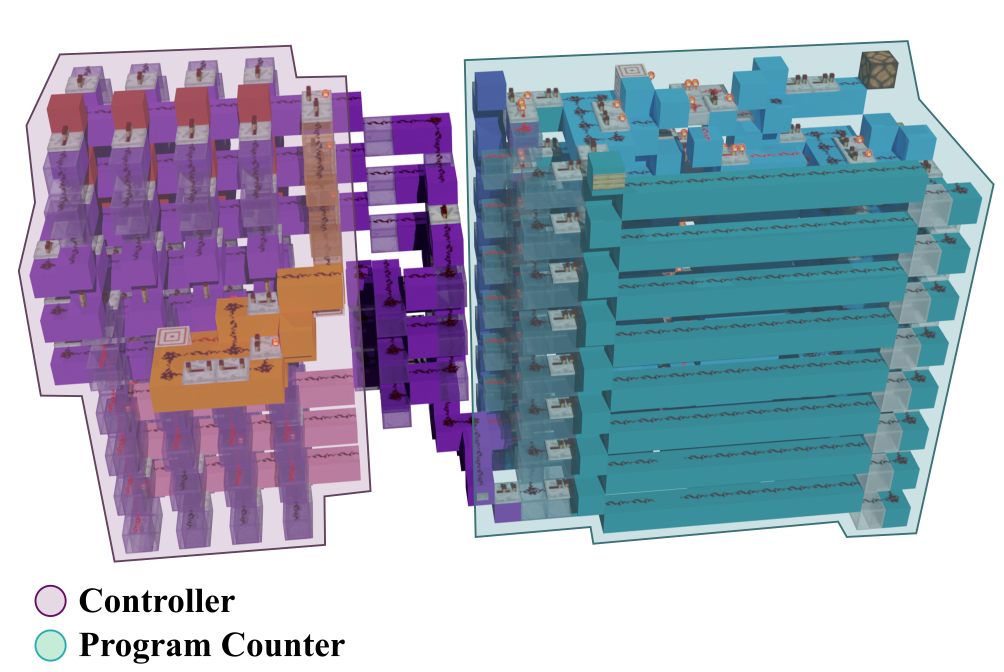
\includegraphics[width=0.55\textwidth]{Figures/FlagsPC_1-small.png}
        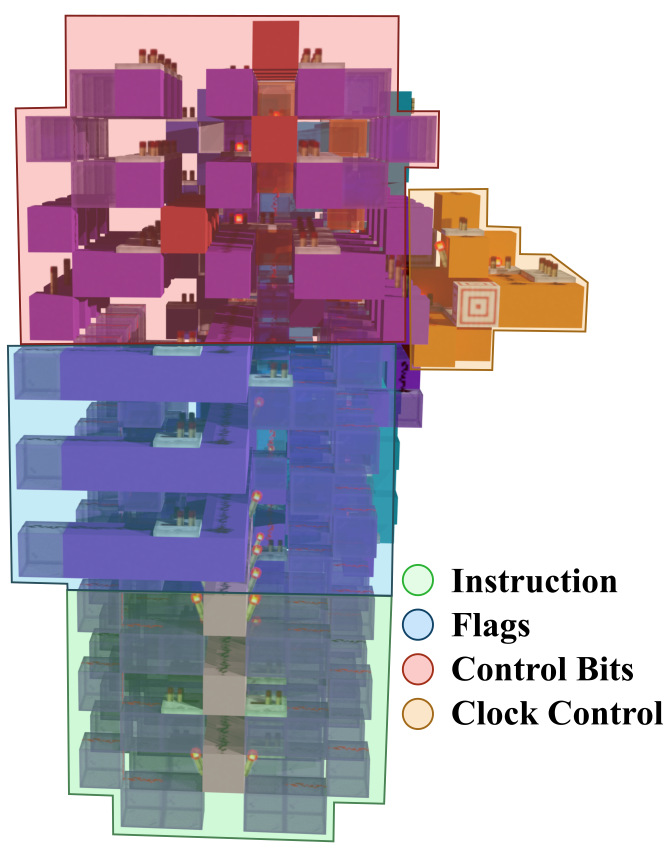
\includegraphics[width=0.35\textwidth]{Figures/FlagsPC-small.png}
        \caption[Program Counter]{The full program counter on the left and an overview of the controller on the right}
        \label{fig::FlagsPC}
    \end{center}
\end{figure}
Two separate modules make up the program counter. The main module is a simple 8-bit synchronized addition module. The output of the counter feeds back into itself in order to store its current state without the need of further registers. This is visible in Figure \ref{fig::FlagsPC} on the left image as the lines in front that create a loop in the blue module. This setup makes incrementing the counter by one a straightforward process by setting the carry bit in the lowest addition unit to 1. To set the state of the PC to any arbitrary 8-bit value, the loop is temporarily interrupted to reset the PC while at the same time the new value is given as an input. It is important to note that the carry bit, or any incoming data to the PC, must be a short pulse of exactly 5RT. Otherwise, the program counter will start oscillating its bits on and off due to the nature of the loop. The second module is the controller and takes in both the flags from the ALU and the 3-bit instruction code from the Instruction Decoder. It utilizes a decoder where the instruction is matched with the required flag states to give an output. This decoding unit can be seen on the right side of Figure \ref{fig::FlagsPC}, where the instruction code is input in the bottom in pink, while the flag states are input in the middle in purple. Each conditional jump instruction only considers the flags that are important to it, while the others aren't connected to its decoding unit. The output for each instruction can either tell the PC to increment or to jump to a given address by setting control bits that get sent to the PC. For example, a JIN (jump if negative) instruction would be received from the Instruction Decoder as some combination of a 3-bit number. This matches two decoding units, one of which requires the negative flag to be on, the other requires it to be off. When the shortened clock pulse arrives, the controller either gives an increment signal, i.e. enabling the carry bit, when the condition is not met or a jump command by disabling the loop and feeding in the new address. Finally, the clock segment on the right is used to give a short 5RT pulse on both the falling and the rising edge of the clock signal in order to perform both PC operations in the execution of an instruction.

\subsubsection{Branching}
A jump is the equivalent to a branch in a program, like an If-statement, where the program continues on a different line. This is achieved by setting the value of the PC to the desired position in the program. A function call, for example, will always include an unconditional jump to the beginning of the function. The return statement at the end of the function then unconditionally jumps back to where the function was called. If-statements, in this CPU, make use of one of two conditional jump instructions: jump if negative (JIN) or jump if zero (JIZ). The JIZ instruction specifically is used most often in loops, where each iteration the loop counter, the value that keeps track of the number of times the loop is being executed starting at the desired loop length, is decremented by one and the state written to the flags register by the ALU. If the loop counter has reached zero, the JIZ instruction exits the loop to a specified line in the program. The example programs that were run as a demonstration of this CPU, particularly the multiplication in section \ref{ssec::Multiplication}, show this concept of looping a set number of times.

\section{Timing}

\subsection{The Danger Sign Problem} \label{ssec:DangerSign}
The following problem was taken from the book \emph{introduction to computing systems} \cite[Chapter 3.6.6]{danger_sign}.
The danger sign displays an arrow using lights separated into three parts that are controlled individually to indicate a turn to the right. The goal is to have the lights turn on sequentially to the right, i.e. the arrow starts off dark, then the first section (lights 1 and 2) turns on, then the second section (lights 3 and 4) turns on and then the third (light 5), at which point all lights turn back off again. Each step in this process should happen in 1 second intervals. The lamp therefore has four states represented in simple binary as A(00), B(01), C(10) and D(11).
\begin{figure}[ht]
    \begin{center}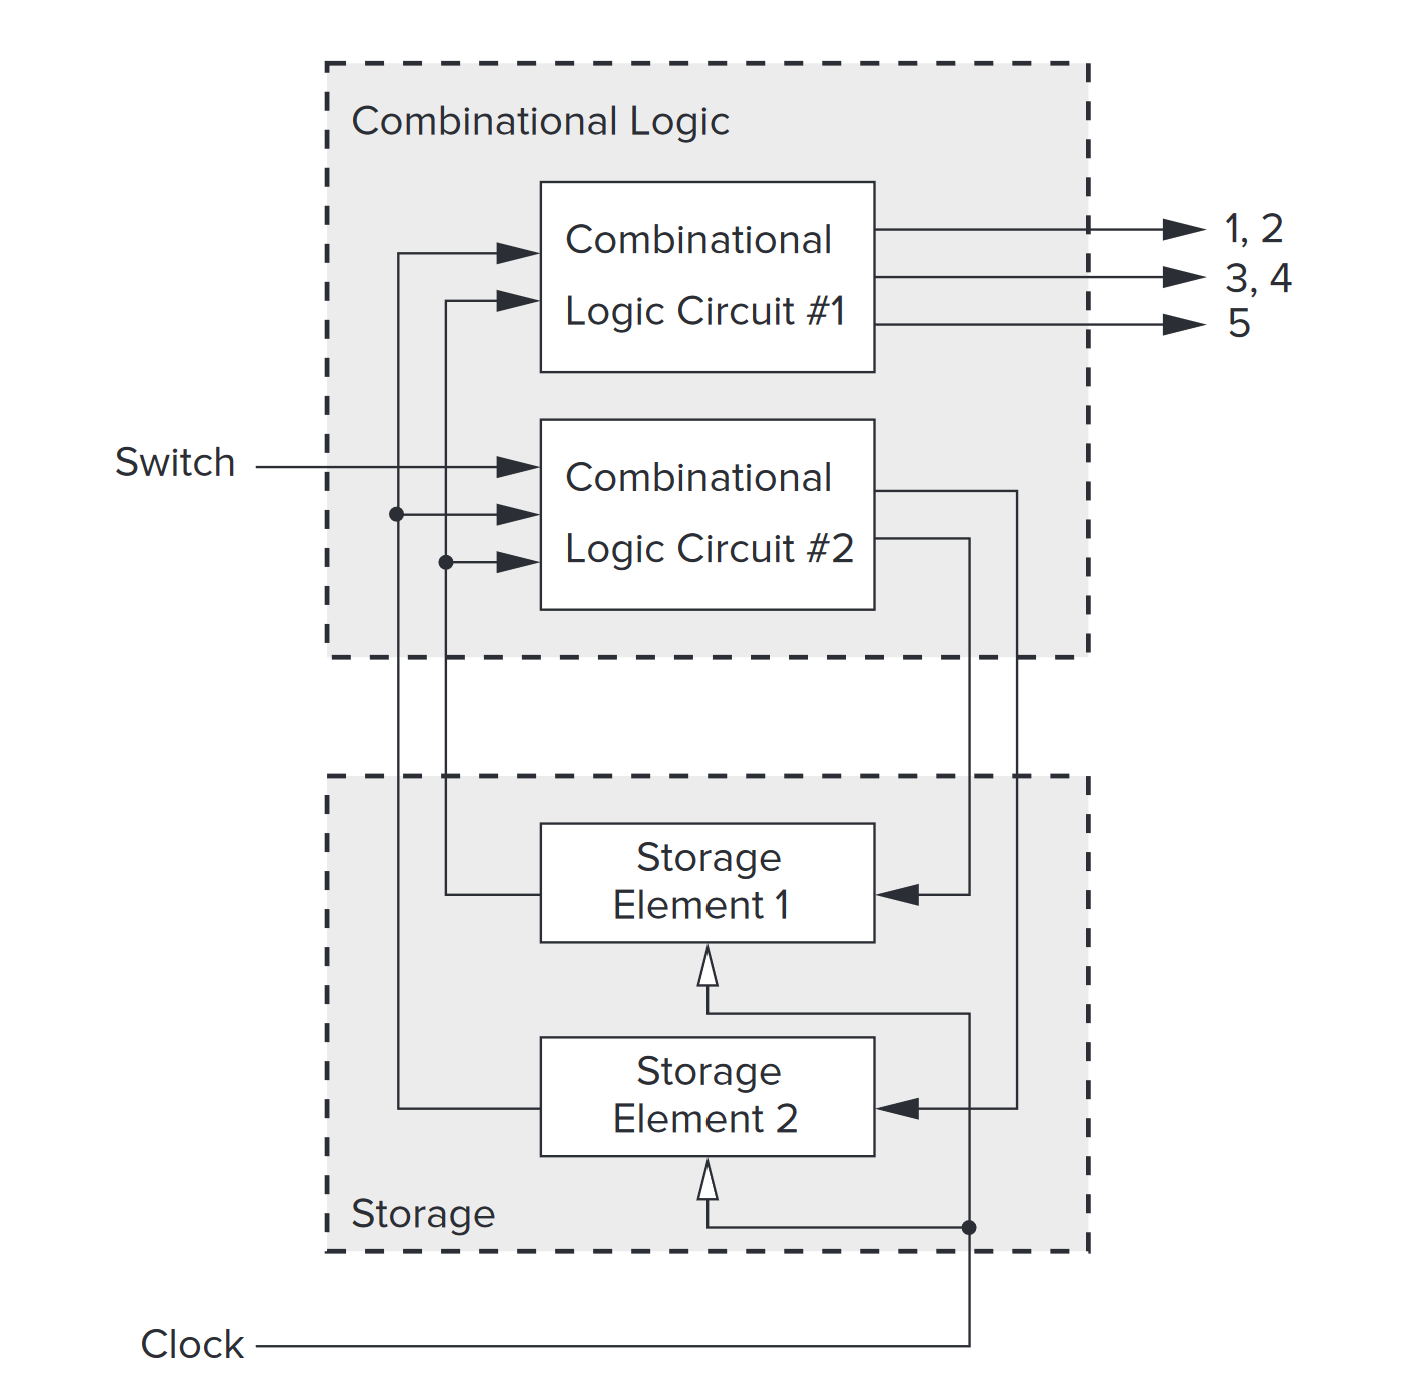
\includegraphics[scale=0.6]{Figures/DangerSignLogicCircuit.png}\end{center}
    \caption[Sequential Logic Circuit]{Sequential Logic Circuit, Source: \cite[Chapter 3.6.6]{danger_sign}}
    \label{fig::DangerSignSequential}
\end{figure}
\newline
Figure \ref{fig::DangerSignSequential} shows the layout of the internals of the controller for the lights. Storage element 1 stores the low bit and storage element 2 stores the high bit. The combinational logic circuit 1 determines which of the lights should be active based on the state of the storage elements. State C(10) for example turns on lights 1 through 4. The combinational logic circuit 2 determines the next state based on the current state, iterating through all states in order. The clock controls the timing of the transition between two states in the storage unit. The choice of what type of storage element to use is critical, as will be apparent later. Starting with \emph{gated D latches} is a good bet, since they are relatively simple in design. If the clock is high, the state of the latch is set to whatever its input state is. If the clock goes low, the latch keeps its current state as is. Additionally, the latch always outputs its current state. The storage elements output their data, the combinational logic controls the lights and outputs the next state back to the storage elements, which, when the clock is high, store that data.
\newline
This approach, however, presents a problem. The time that the output from storage takes to go through the combinational logic and return to storage is significantly shorter than a single clock cycle. Since the clock will still be high when the next state arrives at storage, the gated D latches will receive and store the new data and send their new state to the combinational logic circuits once again. What this means is that the state of the system iterates many times in a single clock cycle and the lights flicker indistinguishably through all possible combinations of A through D, as demonstrated in Figure \ref{fig::TrafficLightClock}. The lights would lose their purpose of showing people the way.
\newline
\begin{figure}[ht]
    \begin{center}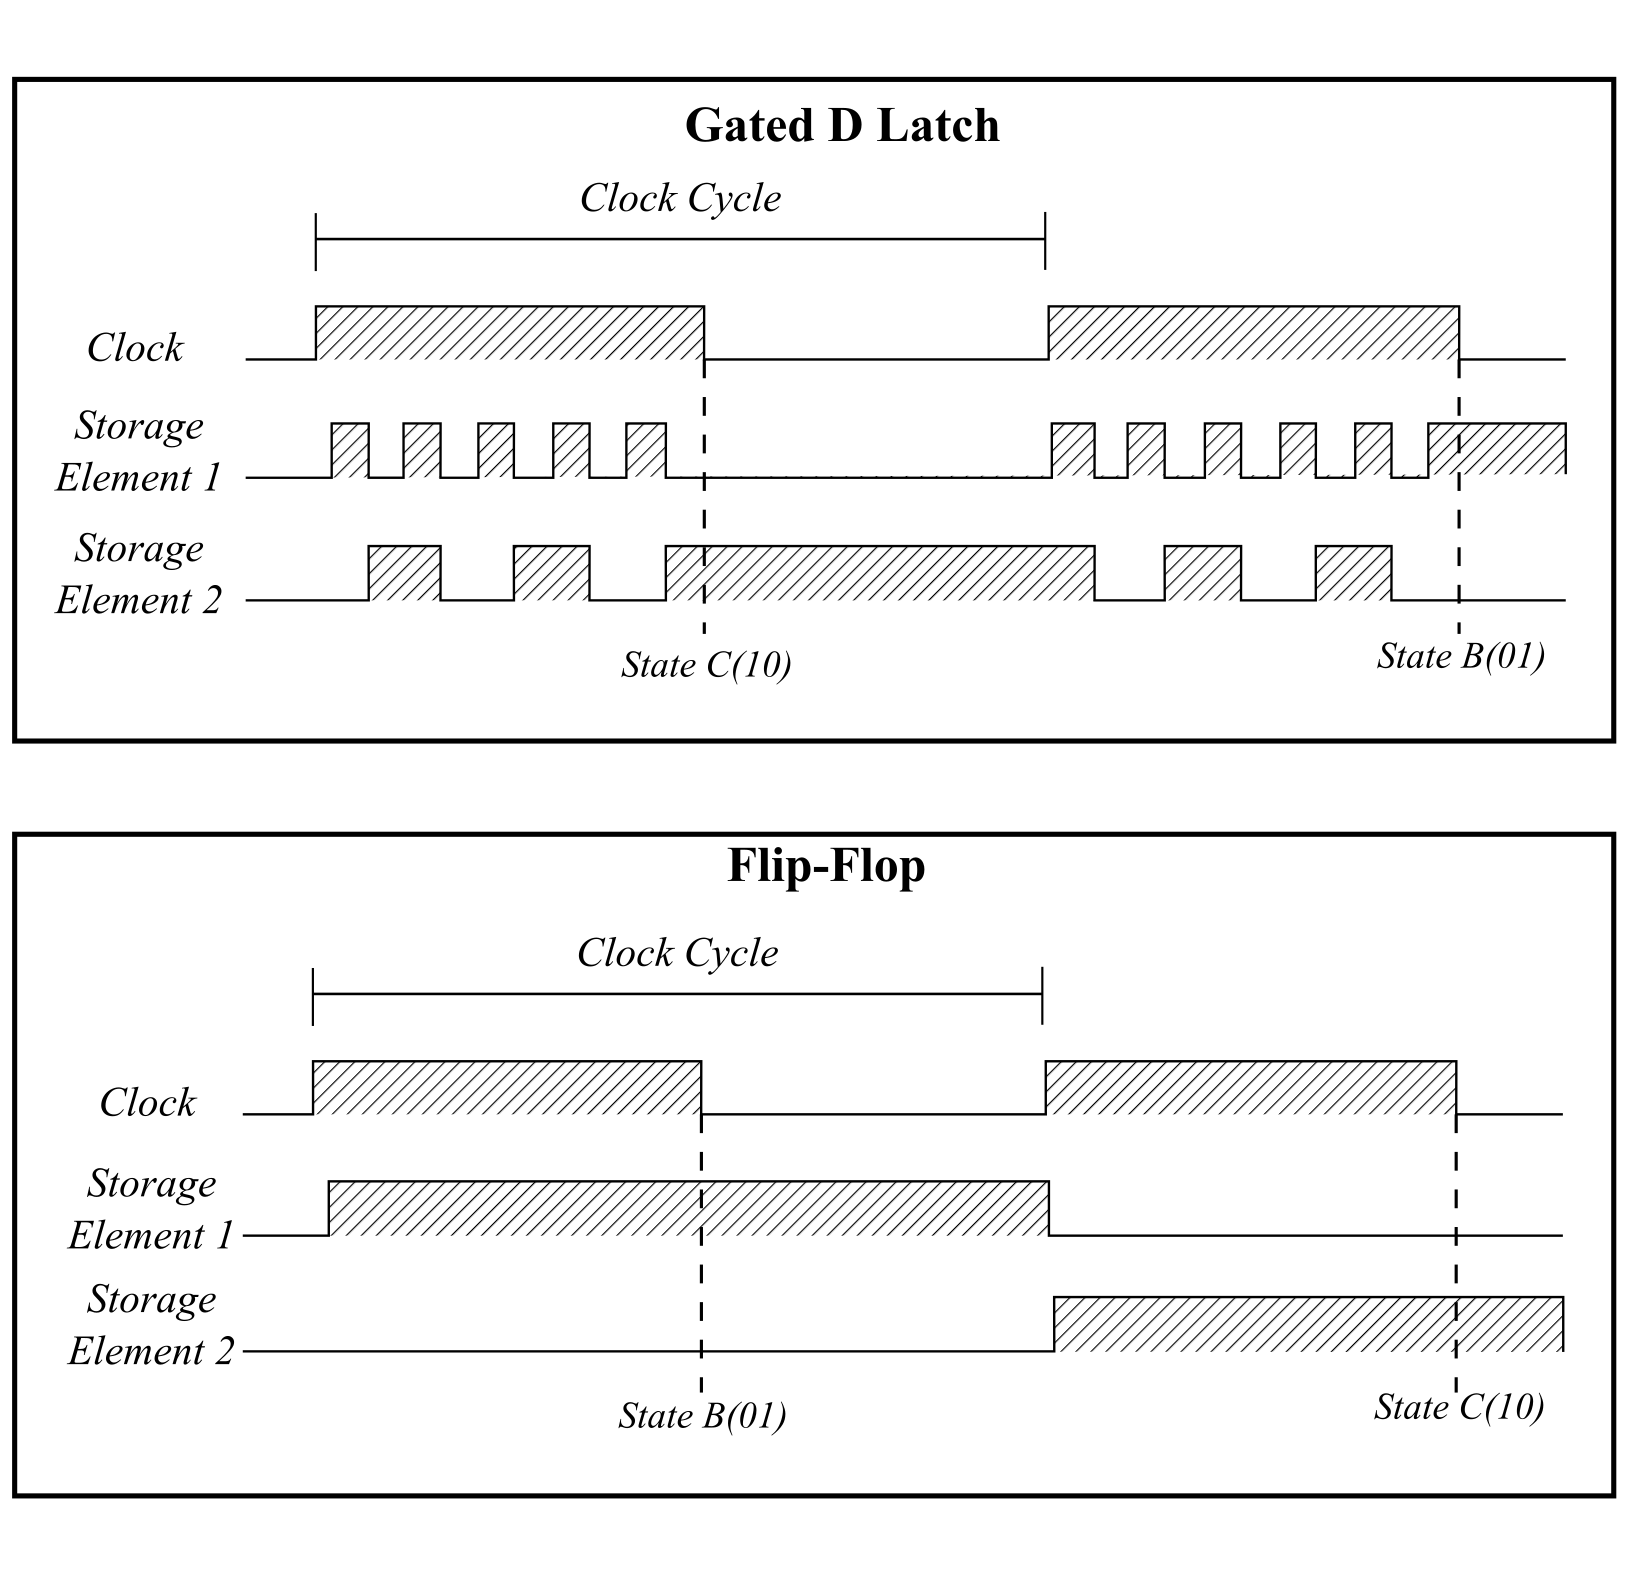
\includegraphics[scale=0.8]{Figures/TrafficLightClock.png}\end{center}
    \caption[Gated D Latches and flip-flops]{Comparing gated D latches and flip-flops}
    \label{fig::TrafficLightClock}
\end{figure}

\subsubsection{The Flip Flop}
\begin{figure}[bp!]
    \begin{center}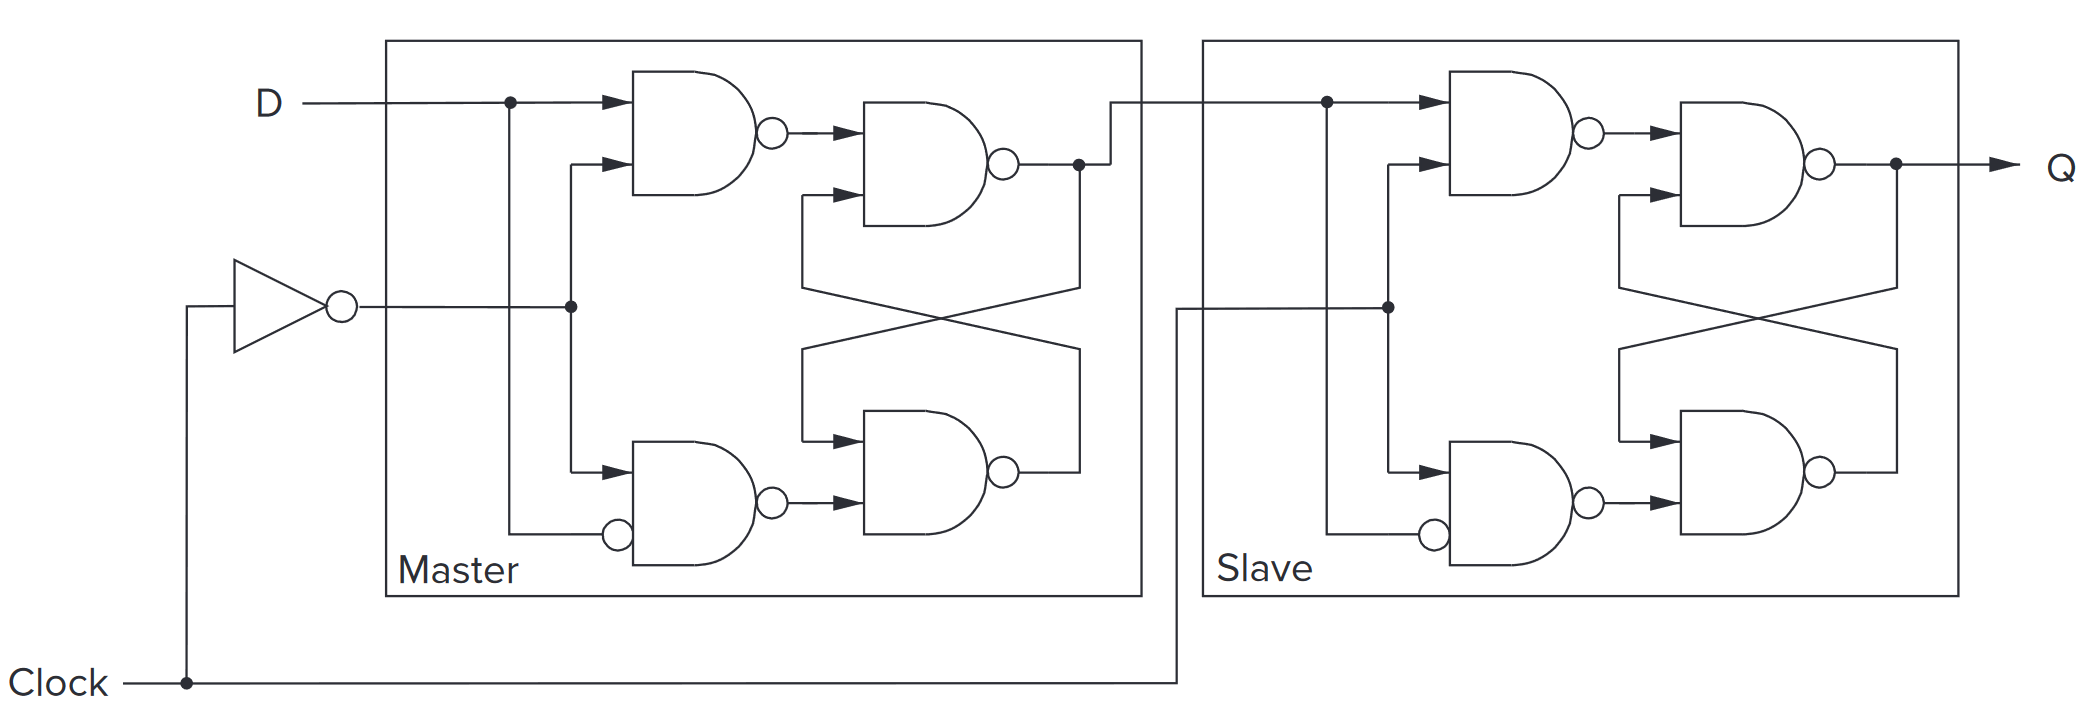
\includegraphics[scale=0.5]{Figures/MasterSlaveFlipFlop.png}\end{center}
    \caption[Master-Slave flip-flop]{A master-slave flip-flop, Source: \cite[Chapter 3.6.6]{danger_sign}}
    \label{fig::MasterSlaveFlipFlop}
\end{figure}
Using a \emph{flip-flop} instead of the gated D latch solves the problem. A flip-flop is a sequential logic circuit which is designed change its state only on the rising or falling edge of the clock cycle, i.e. when the clock transitions from high/low to low/high. This is achieved by setting up two gated D latches in series, where the first one is called the master latch and the second one the slave latch. The slave latch is set up identically to the previous design, so when the clock is high, it changes its state to the data it receives. This data comes directly from the master latch, which is set up inversely to the slave, only changing state when the clock is low. The output of both latches is still continuous. When the clock is low, the master latch stores the next state of the system as computed by the conditional logic circuit 2, but the slave latch, which stores the current state, doesn't change its state to the next state. Only when the clock goes high does the slave latch change its state and stores the next state. This time the master latch doesn't process the next state and so the slave will not change its state any further. In each clock cycle the system's state will only increment once.

\subsubsection{Short Pulse Write}
The problem of data being written too quickly is not uncommon and actually posed some significant problems during the development phase of this project. Minecraft provides the player with more possibilities for such issues. For example, a fix that should only be used in smaller circuits is to extend the time that the signal takes to make it back to the gated D latch by introducing some repeaters. The benefits of this method are a more efficient usage of space and easily modifiable delay timings. The reason this shouldn't be used for larger circuits is that slowing down any transmission of data often limits the speed of the entire circuit. Another problem in larger circuits is that storage units will often not receive their data from one source alone, but from many sources which all have take different amounts of time to process data and for that data to arrive at the storage units, making it very hard to time everything correctly. It is the easiest solution to come up with and to implement in a small circuit, but probably the worst option to choose for the aforementioned reasons. A common approach used in this project is to shorten the length of the incoming pulse to be only as long as the storage element requires to write the data. This can be achieved by using a pulse-width limiter as described in section \ref{ssec::Components}, where a comparator and a repeater set to the required delay generate the necessary pulse length once the clock signal goes high. As long as the data from every possible source arrives at the storage units before the clock goes high, the correct data will be written at the time the clock goes high. Using this method, by the time the combinational logic sends the next state to the storage elements, they will no longer write any further data for the remainder of that clock cycle.
The solution presented in the danger sign problem also applies to Minecraft, and is a very elegant solution, though, when scaled up, uses space significantly less efficiently than the shorter pulse, because each bit to be stored would require two gated D latches instead of a single pulse-width limiter for the entire storage array.

\subsection{Program Counter Difficulties}
The nature of the program counter using a comparatively slow loop brings forth a set of requirements to not fall into a state of oscillation. The loop consists of the addition module and the lines that loop back to the input to store the current state. As soon as data gets to the PC, the signal propagates through the module and takes about 5-6RT to reach the input again and settle into a stable state. The problem arises when the length of the signal is either too short or too long. When the signal is too short the data doesn't make it through the module in time to reach the beginning again before the signal turns off. What this means is that part of the module is in the previous state while the rest is in the new state. This arrangement of states then loops around in a circle. This primarily happens when the program counter controller, which matches the instruction with the required flags and controls the input to the PC, has the wrong pulse-width limiter settings or when the incoming data, either the new address or the instruction code, arrives too late and is subsequently cut off too early. The signal being too long is only a problem for the carry bit and happens when the pulse-width limiter is set up incorrectly. The carry bit is unique in the way that it only affects the lowest bit and not itself. When the lowest bit and the carry bit are on, the lowest bit carries the bit up to the next layer and turns off, at which point the carry bit, which in this situation is still on, turns on the lowest bit once again. This results in a continuous counter while the carry bit is on. Either the PC starts oscillating or ends up in a wrong state. This situation is very similar to that of Section \ref{ssec:DangerSign} and could have been solved in the same way, but since it is a major change to the implementation of the PC, it was deemed not important enough. In hindsight, using flip-flops to store the state of the program counter would have been a better solution, since it eliminates most timing issues.

All the different possible interactions between components means the time it takes for a signal to arrive can differ by a significant amount, which means the clock signal needs to change only once the slowest signal that can arrive has arrived. Additionally, the faster signals need to stick around long enough for the clock signal to change, or else the PC fails again. A lot of time went into getting the balance of signals right, and every time something went wrong, chances were it was the program counter that failed.

\section{Instruction Set}
The list of instructions, the instruction set, is the function that connects the user to the machine. Through the instructions, the programmer can tell the machine what to do and is the key to the potential of the computer. Creating the instruction set is likely the most important and impactful part of designing a CPU, at least in the eyes of the user. There are many options of instructions and designs that need decisions to be made, and all with their advantages and disadvantages, so that there is no objectively perfect design for all computers. The instruction set used in this CPU, as in Table \ref{tab::InstructionSet}, was designed with the help of the book \textit{Computer Architecture}, \textit{A Quantitative Approach} \cite[Appendix A]{Computer_Architecture}, though the ideas presented in the book were not followed strictly and adapted to what seemed a better or easier implementation. The choices made for this CPU are sometimes also remnants from a previously built prototype and include some flaws that could have been avoided if more thought and time had been put into them. Nevertheless, the instruction set allows for theoretically any program to be implemented, though the CPU is limited to its 8-bit range.

\begin{table}[ht]{\small
    \caption[Full Instruction Set]{\textbf{Full Instruction set.} A, B and X are assumed to be registers, while I is an immediate formed by A and B, where B is the higher and A the lower valued half of the byte. The Flags column indicates wether the flags register is updated during the operation. Additionally, A must always be an even numbered register, while B must always be odd numbered}
    \label{tab::InstructionSet}
    \begin{tabular}{|l|c|c|r|c|c|l|}\hline
        Instr. & Result & A & B & Flags & Opcode & Description\\ \hline \hline
        LDA & X & I &      & no  & 0001 & Loads I into Register X\\ \hline
        STR & X & I &      & no  & 0010 & Stores Register X into Address I\\ \hline
        MOV & X & A & or B & no  & 0011 & Moves Register A/B into X\\ \hline
        ADD & X & A & B    & yes & 0100 & Adds A and B into X\\ \hline
        SUB & X & A & B    & yes & 0101 & Subtracts B from A into X\\ \hline
        INC & X & A & or B & yes & 0110 & Increments A/B into X\\ \hline
        DEC & X & A & or B & yes & 0111 & Decrements A/B into X\\ \hline
        AND & X & A & B    & yes & 1000 & Binary AND A and B into X\\ \hline
        ORA & X & A & B    & yes & 1001 & Binary OR A and B into X\\ \hline
        NOT & X & A &      & yes & 1010 & Binary NOT A/B into X\\ \hline
        BSL & X & A & or B & yes & 1011 & Bit-shift-left A/B into X\\ \hline
        BSR & X & A & or B & yes & 1100 & Bit-shift-right A/B into X\\ \hline
        JMP &   & A & or B & no  & 1101 & Jumps to instruction A/B\\ \hline
        JIN &   & A & or B & no  & 1110 & Jumps to instruction A/B if negative flag\\ \hline
        JIZ &   & A & or B & no  & 1111 & Jumps to instruction A/B if zero flag\\ \hline
    \end{tabular}}
\end{table}

\subsection{Instruction Set Architecture}
The way the executing part of the CPU interacts with memory is the defining feature of different Instruction Set Architecture Classes, and is closely linked to the CPU Architecture, as discussed in Section \ref{ssec::Architecture}. Figure \ref{fig::ISA} shows a simple diagram of the four main architecture classes. The stack and accumulator classes both involve implicit operands, i.e. operands that are used without the need to be specified. An operand is part of an expression, like a value or a register containing a value or acting as a destination for the result. The stack's operands are the two operands on top of the stack (TOS), while the accumulator holds one operand implicitly and the second operand is taken explicitly from the instruction. The usage of implicit operands limits the flexibility of the program, especially in a stack format, since expressions must be evaluated in one specific order, as the stack can only hold values in one order. The other two architecture classes make use of general purpose registers (GPR). This means none of the operands are implicitly given and their use must always be stated explicitly. The difference between register-register and register-memory classes is the relationship to memory: register-register architecture only allows registers as operands, which need to be loaded into registers and stored into memory separately and is thus often referred to as load-store architecture, while register-memory architecture takes one of its operands directly from memory, just as the accumulator class, while still specifying which register to choose the first operand from. The usage of GPR allows for easier storing of variables and reserving certain registers for expression evaluation, meaning e.g. expressions can be evaluated in any desired order. Another distinction between GPR architectures is the maximum number of allowed operands: a three-operand format uses one result register and two source registers, while the two-operand format uses one of the two operands as both source and result register. For this project, the load-store architecture class with a three-operand format was chosen, due to the ease of implementation, not needing an additional interface with memory for one of the operands during an operation and highest amount of flexibility of the different classes. Another advantage of load-store architecture is a fixed-length instruction, which was very important for the hardware implementation so that the modified Harvard architecture, as discussed in section \ref{ssec::Architecture}, could be followed. This choice does however increase the complexity of a compiler, since there isn't a simple step-by-step approach as with, for example, the stack architecture, where each expression uses a predictable series of pushes and pops. Unlike the GPR classes, stack architecture is not very code dense. A compiler for register architecture classes needs to keep track of what register is reserved for what purpose and holds what information. The modern approach to instruction set architecture classes is the load-store method, as is used in ARM, SPARC and RISC-V architectures, precisely because of the high flexibility it allows.

\begin{figure}[ht]
    \begin{center}
        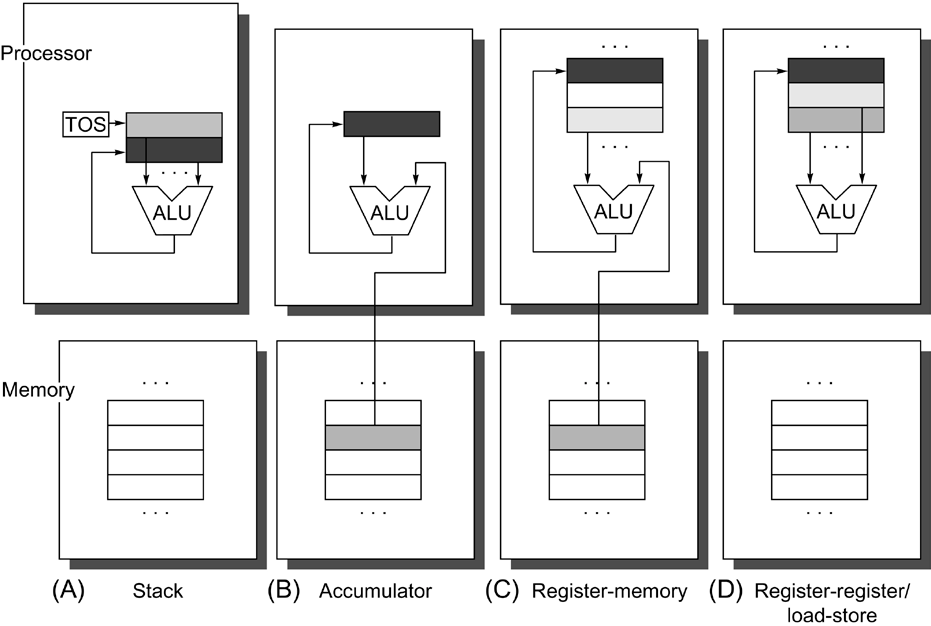
\includegraphics[width=0.8\textwidth]{Figures/ISA.png}
        \caption[Instruction Set Architecture Classes]{Instruction Set Architecture Classes, Source \cite[Figure A.1]{Computer_Architecture}. Both in (A) and (D), the operands can only be transferred to Registers/stack via separate instructions: push and pop for (A) and load/store for (D). (B) and (C) interface with memory directly to perform ALU operations.}
        \label{fig::ISA}
    \end{center}
\end{figure}

\subsection{Addressing Modes}
\begin{table}[bp!]
    \caption[Addressing modes]{A selection of four basic, common addressing modes}
    \label{tab::AddressingModes}
    \begin{center}
        \begin{tabular}{lll}
            Addressing mode & Example Instruction & Meaning \\ \hline
            Register & ADD 0r3 0r2 0r 1 & Regs[3] $\leftarrow$ Regs[2] + Regs[1]\\ \hline
            Immediate & LDA 0r2 0d42 & Regs[2] $\leftarrow$ 42\\ \hline
            Register Indirect & LDA 0r2 0r4 & Regs[2] $\leftarrow$ Mem[Regs[4]] \\ \hline
            Memory Indirect & LDA 0r2 0r4 & Regs[2] $\leftarrow$ Mem[Mem[Regs[4]]]\\ \hline
        \end{tabular}
    \end{center}
\end{table}
Memory addressing covers the way in which the operands in a given instruction are interpreted. There is a variety of different ways an operand can be used to get the desired address or value, four of which are shown in Figure \ref{tab::AddressingModes}. The two most basic addressing modes are Register and Immediate mode, which are also the only two used in this project. Register mode takes in all the operands as register addresses, where the values inside the registers are used for the operation. Immediate mode takes in one immediate (here an 8-bit value) and a register to be used for the operation. These two modes allow for simple use and implementation, but they do bottleneck the programmer in some scenarios. Say, for example, one wants to calculate a simple addition, then store it in memory and later on retrieve this value. Values can easily be stored into registers in the form of an immediate using the LDA command, where the result register and the value are specified using the Immediate addressing mode. Calculations are done using register mode in the three-operand format, specifying one result and two sources. Storing the value in memory uses the Immediate format once again to specify the result address in memory as the immediate and the source register. But retrieving any stored value using only register or immediate mode isn't much of a possibility without workarounds. In fact, the storing only works because of a workaround, where the register and memory addresses are swapped in the instruction to accommodate their different sizes. Ideally, both the store and load instruction should use the register indirect or even memory indirect modes in order to facilitate more flexibility for a program. It is still theoretically possible to store and retrieve values, despite the implementation, but it would require the program to reprogram its own load/store instruction with the new value, i.e. changing e.g. \textbf{LDA 0r2 0d42} to \textbf{LDA 0r2 0d64}, instead of pointing to the stored value in memory.

\subsection{Encoding the Instruction Set}
Finally, the instruction set must be encoded into at most 16 bits, or two bytes, so that each instruction can be stored in two memory units. This maximum value allows for any instruction to be executed in one clock cycle and is still compact enough to be practical. Two arrangements of how to divide up the 16 bits are displayed in Figure \ref{fig::InstructionEncoding}, and they depend on which operand format is chosen. A three-operand format requires the 16 bits to be divided up equally, with four bits for each operand and the opcode, while a two-operand format allows some extra flexibility for the length of the opcode and thus allow for more instructions or even make multiple instruction addressing modes for each instruction possible. Ultimately, the first variant was chosen to facilitate a three-operand format since, at the time, it seemed to make the most sense. In hindsight, the two-operand format, in addition to using the register indirect addressing mode as part of the possible choices, would have been the smarter choice, but since an earlier prototype of this CPU was already using the first encoding, that choice stuck for the project. The layout of where each operand is encoded is also a remnant of the previous prototype and is addressed in more detail in section \ref{ssec::InstructionLayout}. The limit of 4 bits for the instruction means there can be at most 15 instructions. The opcode "0000" was ignored to get rid of an edge case that may have required an additional workaround. Each instruction has its addressing mode hardwired, where load and store use the Immediate and the other 13 instructions use the Register addressing mode. This limitation has a significant effect on the flexibility when programming, but does reduce the complexity for the assembler (section \ref{ssec::Assembler}) slightly, since it doesn't have to consider different addressing modes for the same instruction.

\begin{figure}[h!]
    \begin{center}
        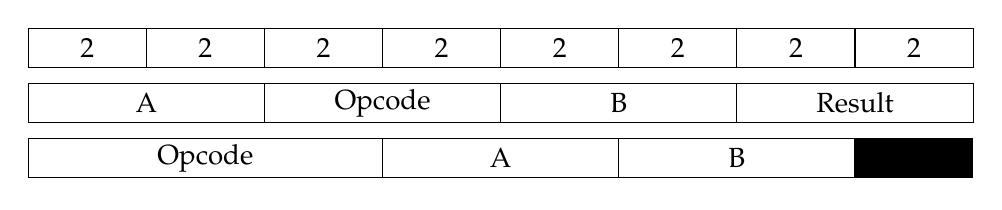
\begin{tikzpicture}
            \draw (0,0.2) rectangle (1.5,0.7) node [midway] {2};
            \draw (1.5,0.2) rectangle (3,0.7) node [midway] {2};
            \draw (3,0.2) rectangle (4.5,0.7) node [midway] {2};
            \draw (4.5,0.2) rectangle (6,0.7) node [midway] {2};
            \draw (6,0.2) rectangle (7.5,0.7) node [midway] {2};
            \draw (7.5,0.2) rectangle (9,0.7) node [midway] {2};
            \draw (9,0.2) rectangle (10.5,0.7) node [midway] {2};
            \draw (10.5,0.2) rectangle (12,0.7) node [midway] {2};
            \draw (0,0) rectangle (3,-0.5) node [midway] {A};
            \draw (3,0) rectangle (6,-0.5) node [midway] {Opcode};
            \draw (6,0) rectangle (9,-0.5) node [midway] {B};
            \draw (9,0) rectangle (12,-0.5) node [midway] {Result};
            \draw (0,-0.7) rectangle (4.5,-1.2) node [midway] {Opcode};
            \draw (4.5,-0.7) rectangle (7.5,-1.2) node [midway] {A};
            \draw (7.5,-0.7) rectangle (10.5,-1.2) node [midway] {B};
            \fill[black] (10.5,-0.7) rectangle (12,-1.2);
        \end{tikzpicture}
        \caption[Instruction Encoding]{Two possible instruction encodings using 16 bits. The top row shows the length for 2 bits. The middle row displays the layout for the three-operand format and the bottom row displays the two-operand format}
        \label{fig::InstructionEncoding}
    \end{center}
\end{figure}

\section{User Interface}
Aside from flying into the CPU itself and examining it or manually, carefully powering redstone lines there is no way to get or set any data from memory. To program the CPU and execute a program, a User Interface (UI) is required. Since the UI is usually not a very intrusive construction, it doesn't affect the function of the CPU and can thus be added on to without needing to consider every other component of the CPU. The implemented UI consists of three levels, each level up decreasing the amount of work for the user. The first level is a direct connection to the memory and clock of the CPU, while the second and third level use external python programs and are purely quality of life features but make the process of creating and writing programs significantly easier.

\subsection{Control Panel}
\begin{figure}[hb!]
    \begin{center}
        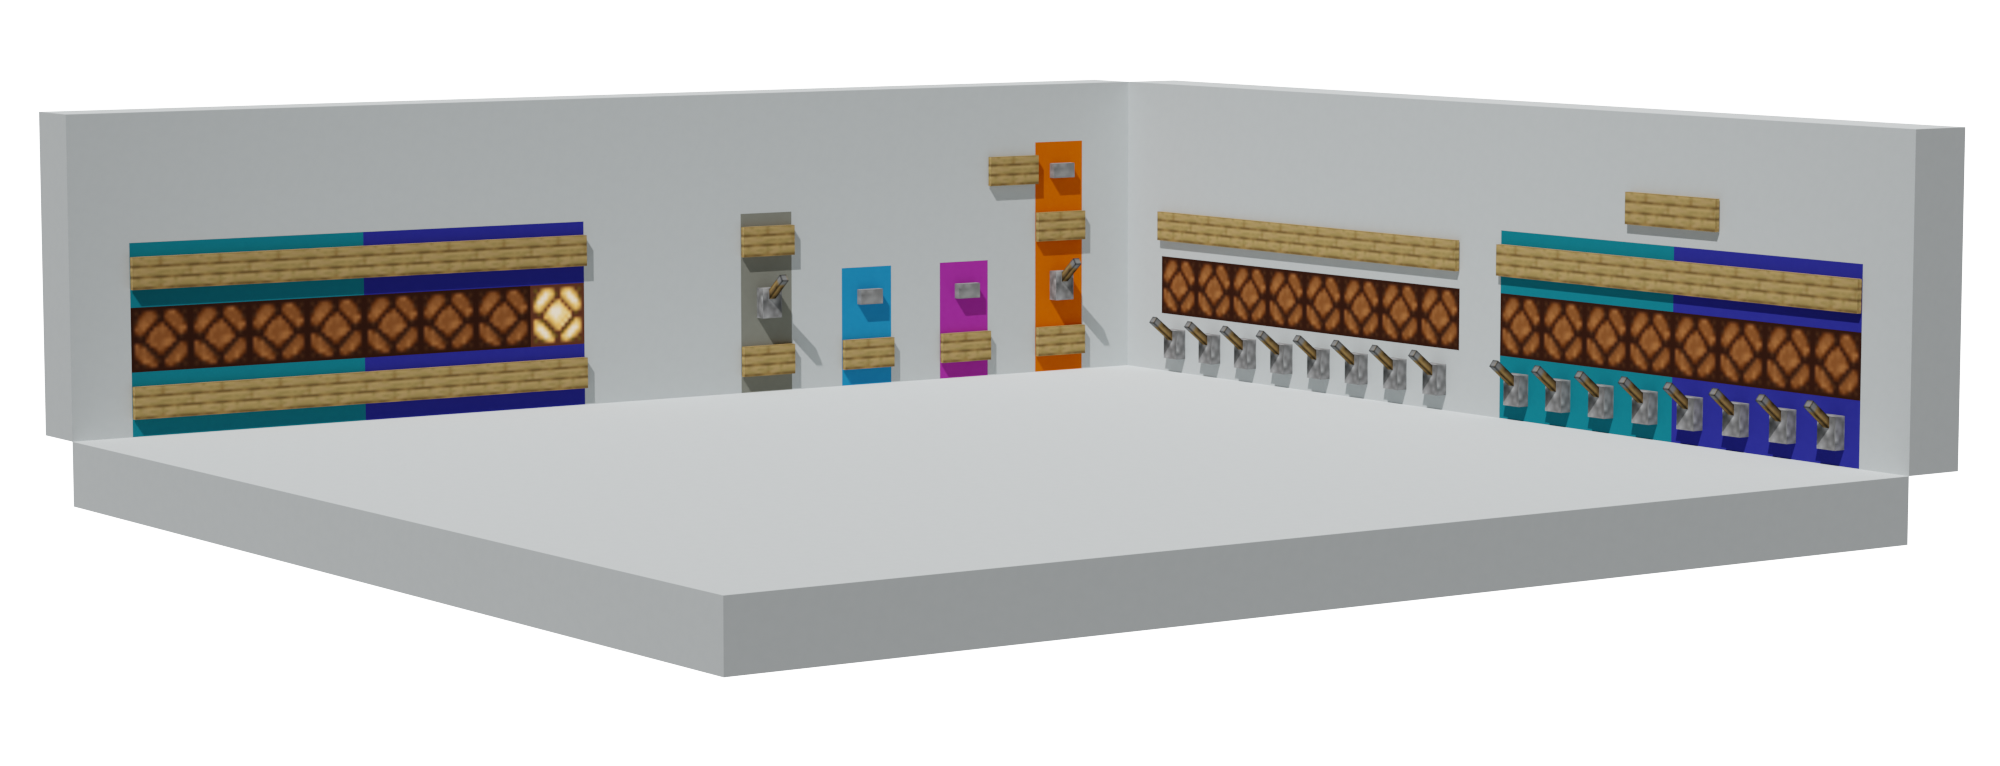
\includegraphics[width=0.8\textwidth]{Figures/ControlPanel.png}
        \caption[Control Panel]{Control Panel (left to right): output, I/O toggle, Reset PC, PULSE UPDATE, Clock, Address, Input}
        \label{fig::ControlPanel}
    \end{center}
\end{figure}
The control panel gives the user a lot of direct control. The biggest area is taken up by the input and output signals while a relatively small area is for some buttons and levers to control various features. The input module consists of an 8-bit address and an 8-bit value, clearly visible on the right wall in Figure \ref{fig::ControlPanel}. Each individual bit can be toggled on or off by hand while the current state of the input is displayed using redstone lamps. The values are connected directly to the RAM module and, with the push of the PULSE UPDATE button, are written to the specified address. The PULSE UPDATE button (in magenta) enables the address signal for a brief moment, allowing the address to be sent into the RAM and write the given data. This part uncovered a fairly significant issue with the timing for when the address lines arrive in each memory unit. Mainly, since the memory unit at address zero would always read zero while no address is present, an additional signal gets sent to that unit to deactivate the decoder until the write pulse arrives, and this signal needs to arrive at precisely the correct time due to the very short amount of time that the address gets sent through memory. This should merely be a matter of counting the redstone ticks for the signals to arrive, but it took an unreasonable amount of time to fix. As a sidenote, during testing larger programs it turned out that somehow quite a few connections were severed, i.e. a single block was missing, and thus some data never got written into memory or read out of memory. Some of these connections again took a large amount of time to discover, which happened mostly when a program began showing nonsensical values. The output module uses the same address bar as the input, but doesn't require any update button. The address feeds into the same line as the PC, so during execution each instruction is shown on the output panel. When reading specific addresses, the PC can be reset to not interfere with the address. Then there is an I/O On or Off lever (in gray) which can disable the input and address, a Reset PC button (in light blue) that sets the program counter to zero and the clock interface where the clock can be turned on or off to cycle continuously or where, by press of a button, the clock can cycle only once (in orange). These lines require little to no additional logic and connect directly to their respective component.

\subsection{Disc Reader}
\begin{figure}[bp!]
    \begin{center}
        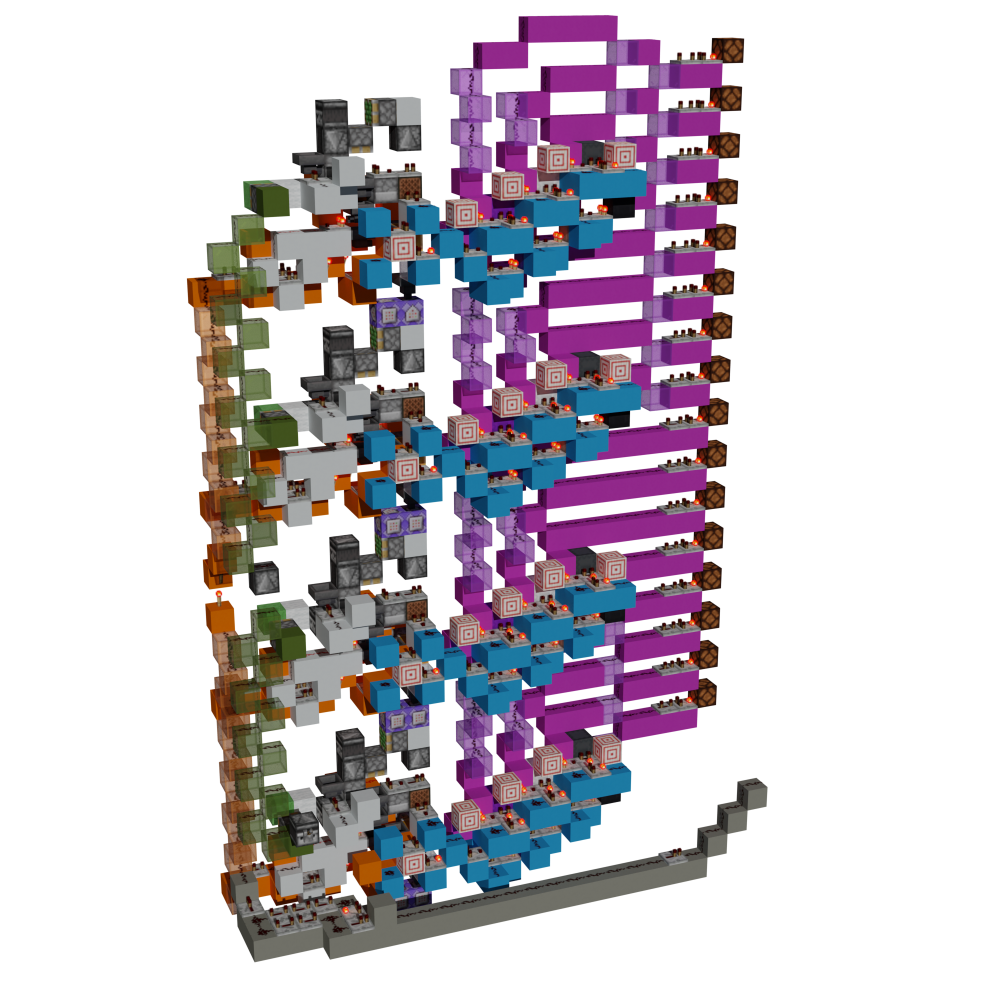
\includegraphics[width=0.48\textwidth]{Figures/DiscReader-small.png}
        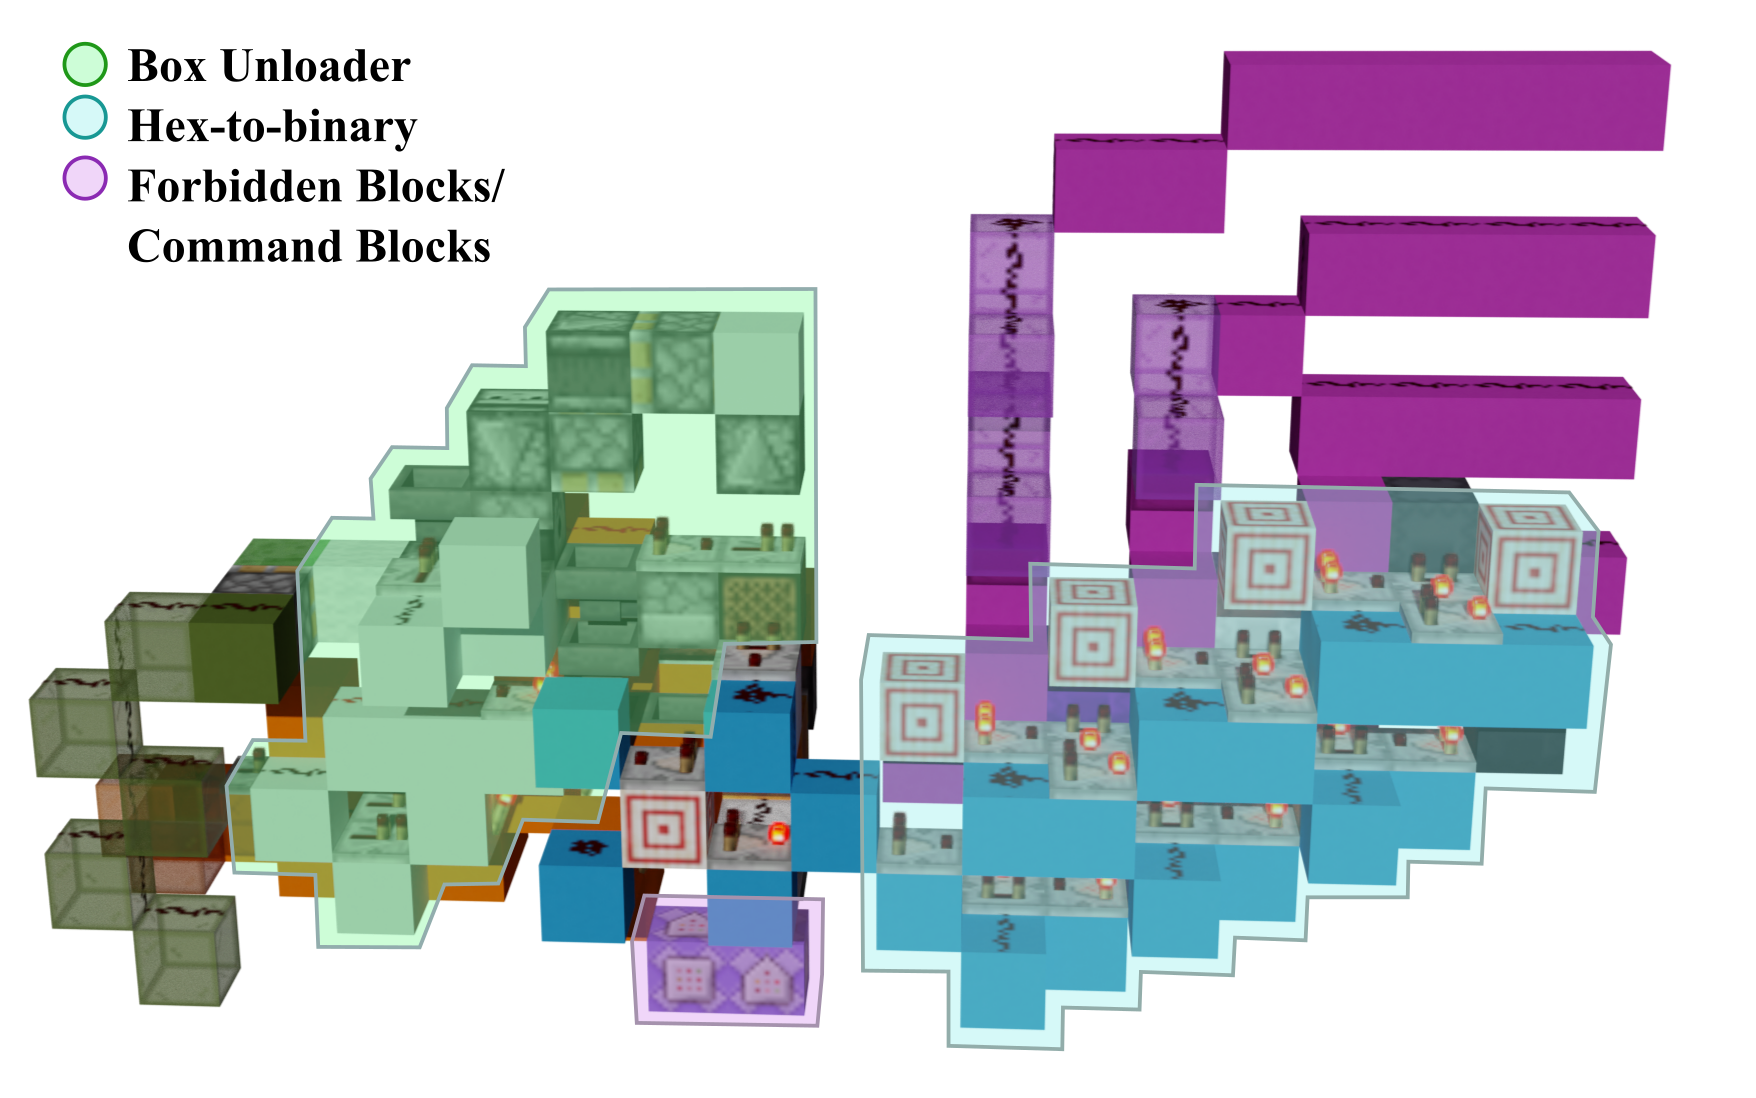
\includegraphics[width=0.48\textwidth]{Figures/DiscReaderUnit.png}
        \caption{Disc Reader}
        \label{fig::DiscReader}
    \end{center}
\end{figure}
Minecraft has another form of data storage neatly implemented though hidden in plain sight: Music discs and chests. Up until recently, this idea would have been complete nonsense, but in the 1.20 update in the summer of 2023, two technically small changes were made. First, each music disc, of which there are slightly more than 15 different versions, outputs a redstone signal with a strength readable by a comparator when it's playing inside a jukebox. Second, jukeboxes can be interacted with by redstone components, namely droppers to insert and hoppers to remove the music disc. This way, a series of music discs can be stored in a chest, or shulker box, which is a chest that can be placed and broken with redstone components, and continuously fed into a jukebox and their respective signal strength read out. Since the signal strengths range between 1 and 15, they encode hexadecimal values and can be decoded into their binary representation in four bits. A zero, which has no music disc, is represented by a stick and is filtered out right before it is pushed into the jukebox, decoding into nothing and thus a zero. Four music discs can therefore be used to store one byte of memory and its address and eight discs make up one full instruction. The decoder works by iteratively checking if each digit fits into the strength of the disc. First the value of 8 is checked to fit, then the value of 4, then 2 and finally 1, while each fitting value is subtracted from the value before the next check. Figure \ref{fig::DiscReader} \space shows the decoder units in blue. The full disc reader is built up of four such decoders, plus an unloading station for the shulker boxes (in white) and a clock (in gray) that sends both the PULSE UPDATE signal, the same one as in the control panel, and the signal to decode the next music disc (in orange in the back). There are command blocks, the purple out of place looking blocks below each unloading station, in this module which would and should be viewed very critically in a contraption that is meant to use the tools given to the regular player to achieve a certain goal. Command blocks are very powerful and can single-handedly do nearly anything, being an interface for commands and scripts. However, their purpose in this case is to delete the music discs and sticks as soon as possible to not create any clutter or unnecessary build up of items in a very compact and easy manner.

\subsection{Assembler} \label{ssec::Assembler}
\begin{figure}[bp!]
    \lstinputlisting[language=Python]{Code/ParserSnippet.txt}
    \caption[Parser code snippet]{A code snippet from the Parser}
    \label{fig::ParserSnippet}
\end{figure}
The assembler provides the user with a tool to take an assembly style program and convert it into machine code, i.e. the ones and zeros that the CPU works with. Assembly is the lowest level programming language because it is an almost direct translation of machine code which makes it comparatively easy to convert into machine code rather than a more abstracted language, even a simple one. The assembler processes the code in two steps: tokenizing and parsing. The tokenizer iterates through every character, stores each white-space separated string as a token and automatically determines the type of the token, i.e. an instruction, a register or a decimal/immediate. Additionally, the tokenizer will recognize comments denoted by a "\#" and ignore the rest of that line. Assembly being such a low level language, each line can be evaluated completely in isolation of the other lines (There are certain features that would require the evaluation to keep track of some values, mainly for the branch instructions, but these features are not implemented yet). Once each instruction is tokenized, the parser begins iterating through each line. From this point on, each instruction group has a slightly different way of being parsed, but, in essence, each is the same. Each instruction has an entry in a dictionary and is mapped to a unique instruction code. The arguments are then encoded from decimal to binary and are  checked if they are in the correct position, i.e. all even registers map to A and all odd registers map to B. Each line also gets two addresses as a prefix, for each byte of the instruction, for where in memory the line is stored. This part is only necessary for the function of the next stage, but also helps to debug the program in memory. Figure \ref{fig::ParserSnippet} shows an excerpt of the parser for the instructions in the ALU group. Note that the code was slightly changed for readability and doesn't show the full picture. The full source code is available in the appendix.

\subsection{Binary File to Minecraft}
To load the disc reader, four chests are filled with shulker boxes containing music discs on their respective loading stations. To do this from an external program, a mod called Litematica is used. Litematica allows for the loading and placing of schematics, which can be thought of as a preview or template, and is most commonly used for builders to show them where to place what block. In this case, however, it is used only to place the four chests and their contents in the right spot. In python, the module \textit{mcschematic} provides the tools to easily create schematics. To place a certain block, the function \textit{setblock()}, along with the desired relative position of the block and the block itself, is used. Working with containers and especially containers inside containers is somewhat complex, and there are no easy-to-find guides on how this is works. Luckily, Minecraft provides the user with the ability to use the command \textit{F3 + I} to copy the setblock command for the block the player is looking at to the clipboard. From this, the structure of the block ID can be derived. Figure \ref{fig::minecraftChest} \space shows the block IDs from simple container blocks to containers in containers.
\begin{figure}[h!]
    \lstinputlisting[language=Python]{Code/BlockID.txt}
    \caption{Block IDs for containers}
    \label{fig::minecraftChest}
\end{figure}

Most of the program is responsible for iterating through the binary file and dealing with the necessary offsets and loops required to access the right bits in the binary file. The four bit binary strings are each converted to decimal values between 0 and 15 and then mapped to their corresponding music disc or stick. Finally, each item is inserted into the correct string format and then added to the list of items in the shulker boxes. The code is not very readable nor easy to understand, but it works exactly as intended and thus shouldn't be touched any further, abiding by the ancient law of \textit{If it ain't broke, don't fix it}.

\chapter{Results}

\label{Chapter3}

\section{Programs}

\subsection{Fibonacci}
The Fibonacci series is presumably the most famous sequence of numbers in the world, at least by name. It contains many wonderful properties within itself that reveal themselves under certain circumstances. My personal favorite has to do with phyllotaxis, which is the regular arrangement of leaves or seeds in plants, famously the sunflower seeds in the dark center of the flower, where the Fibonacci numbers are related to the outward arcs that the seeds form when the golden ratio defines the turn fraction between each outward growing seed in the spiral. The concept is best shown in a video by Sebastian Lague: \textit{Coding Adventure: Boids} \cite[Timestamp: 03:03-06:12]{FibonacciSpiral}. The Fibonacci sequence can be expressed through the following formula:
    \[x_0 = 0,\space x_1 = 1\]
    \[x_n = x_{n-1} + x_{n-2} \qquad n \in \mathbb{N} \; [2,\infty[\]
The diagram in Figure \ref{fig::FibonacciDiagram} gives an overview of the function of the program in Appendix \ref{app::Fibonacci}. The final output of the program was 144, corresponding to the 13th value in the Fibonacci sequence (assuming it starts at 0, 1).

\begin{figure}[h!]
    \begin{center}
        {\small 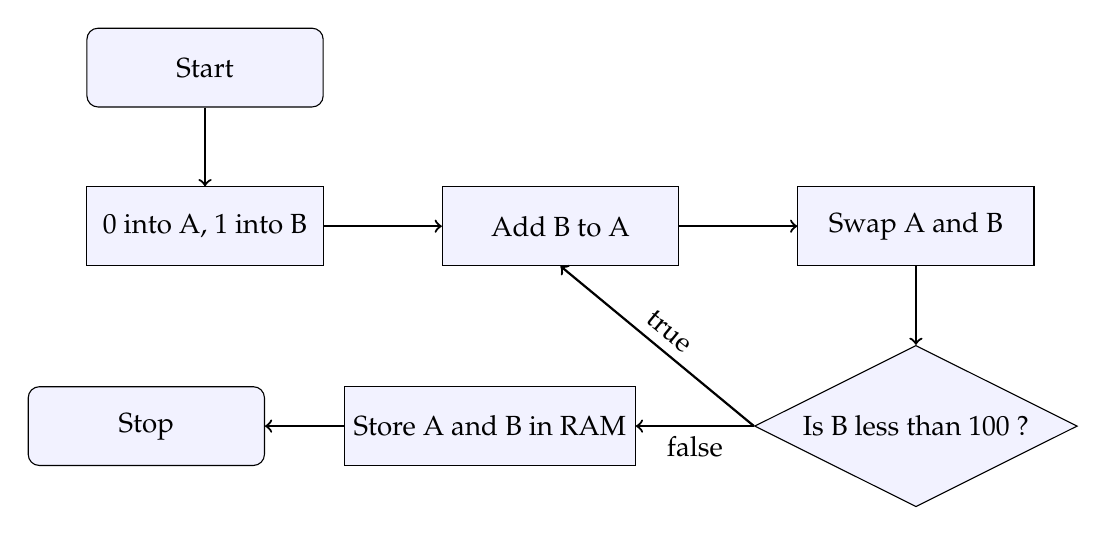
\begin{tikzpicture}
            \node[startstop] (start) {Start};
            \node[process] (load) [below=of start] {0 into A, 1 into B};
            \node[process] (add)  [right=1.5cm of load] {Add B to A};
            \node[process] (swap) [right=1.5cm of add] {Swap A and B};
            \node[decision] (comp) [below=of swap] {Is B less than 100 ?};
            \node[process] (str)  [left=1.5cm of comp] {Store A and B in RAM};
            \node[startstop] (stop) [left=of str] {Stop};
            
            \draw[->, thick] (start.south) -- (load.north);
            \draw[->, thick] (load.east) -- (add.west);
            \draw[->, thick] (add.east) -- (swap.west);
            \draw[->, thick] (swap.south) -- (comp.north);
            \draw[->, thick] (comp.west) -- (add.south)  node [midway,sloped, above] {true};
            \draw[->, thick] (comp.west) -- (str.east)  node [midway, below] {false};
            \draw[->, thick] (str.west) -- (stop.east);
        \end{tikzpicture}}
    \end{center}
    \caption[Fibonacci program diagram]{Program diagram for the Fibonacci sequence that exits once the value is bigger than 100}
    \label{fig::FibonacciDiagram}
\end{figure}

\subsection{8-bit Multiplication} \label{ssec::Multiplication}
Multiplication is a necessity for very many calculations, and is, especially for integers, just a series of additions, which this CPU can handle easily. In binary, multiplication by hand is easier than in decimal, since, for each digit, there are only two possible scenarios: Either the digit is 1, and an addition is performed, or it's 0 and that digit is skipped. Each digit, the summand or the sum needs to be shifted to adjust for the digit value. Figure \ref{fig::MultInBin} illustrates the idea of bit shifting the summand each digit. The procedure shown in the diagram in Figure \ref{fig::MultiplicationDiagram} only outputs correct results for integers whose product is less than 255. The procedure can be modified slightly by shifting the summand right instead of the result left each time to instead multiply two fixed-point decimals represented as $\frac{i}{256}$, i.e. the byte is read out as if divided by 256 while stored as an integer $i$, as is done in section \ref{ssec:LogisticMap}, but is only as accurate as can fit into the eight bits. The non-modified program worked perfectly, outputting the exact value through each test within the limitations. The functionality of the modified version is demonstrated in the next section.

\begin{figure}[h]
    \begin{center}
        \begin{tabular}{ccccc}
            00001011 & $\cdot$ & 00000101 & = & 00000000 \\
            & & & + & 00000000\\
            & & & + & 00000000\\
            & & & + & 00101000\\
            & & & + & 00000000\\
            & & & + & 00001010\\
            & & & + & 00000101\\
            \hline
            & & & = & 00110111
        \end{tabular}
    \end{center}
    \caption[Multiplication by hand]{Multiplication in binary by hand, performed from left to right: 11 $\cdot$ 5 = 55}
    \label{fig::MultInBin}
\end{figure}

\begin{figure}[h]
    \begin{center}
        {\small 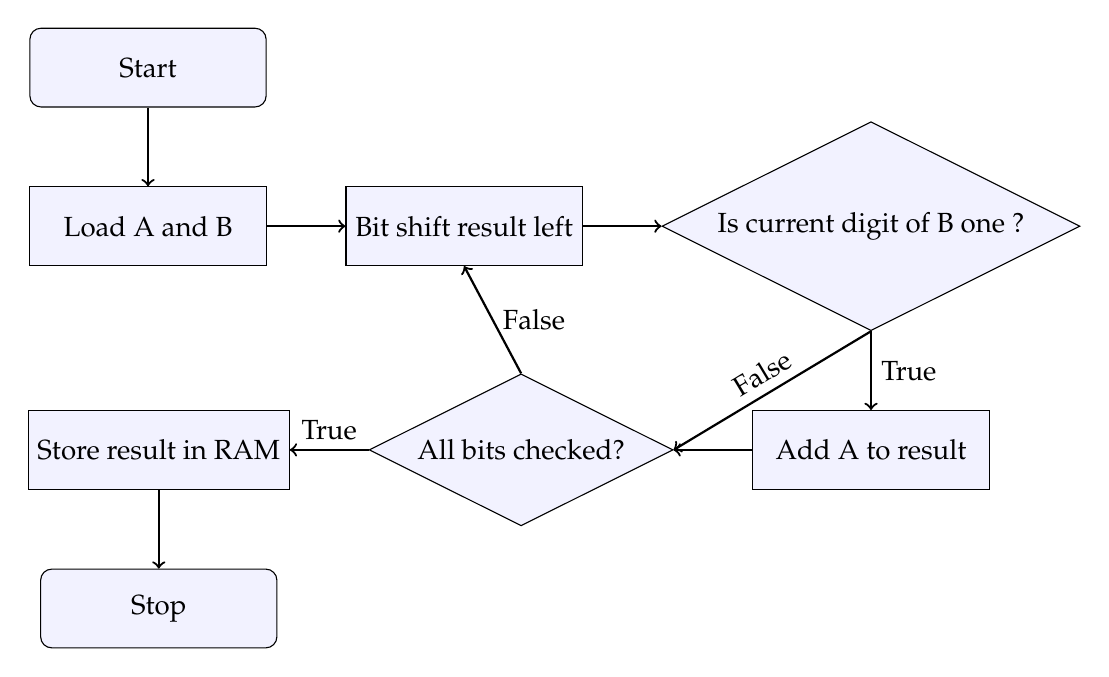
\begin{tikzpicture}
            \node[startstop] (start) {Start};
            \node[process]  (load) [below=of start] {Load A and B};
            \node[process]  (bsl)  [right=of load ] {Bit shift result left};
            \node[decision] (mask) [right=of bsl  ] {Is current digit of B one ?};
            \node[process]  (add)  [below=of mask ] {Add A to result};
            \node[decision]  (loop) [left=of add  ] {All bits checked?};
            \node[process]  (str)  [left=of loop  ] {Store result in RAM};
            \node[startstop](stop) [below=of str  ] {Stop};

            \draw[->, thick] (start.south) -- (load.north);
            \draw[->, thick] (load.east) -- (bsl.west);
            \draw[->, thick] (bsl.east) -- (mask.west);
            \draw[->, thick] (mask.south) -- (add.north) node [midway, right] {True};
            \draw[->, thick] (mask.south) -- (loop.east) node [midway, sloped, above] {False};
            \draw[->, thick] (add.west) -- (loop.east);
            \draw[->, thick] (loop.west) -- (str.east) node [midway, above] {True};
            \draw[->, thick] (loop.north) -- (bsl.south) node [midway, right] {False};
            \draw[->, thick] (str.south) -- (stop.north);
        \end{tikzpicture}}
    \end{center}
    \caption[Multiplication program diagram]{Program Diagram for the multiplication procedure}
    \label{fig::MultiplicationDiagram}
\end{figure}

\subsection{Logistic Map} \label{ssec:LogisticMap}
The Logistic Map \cite{LogMap_Wiki} is an example of how a very simple, iterative equation can display chaotic behavior from small changes in its initial starting condition. It was originally popularized by the biologist Robert May in a paper in 1976 as a model for population behavior. The equation is written
\[x_n = r \cdot x_{n-1} (1-x_{n-1})\]
In the demographic model as per May, $x_n$ represents the ratio between current population to the maximum possible population, while the constant r dictates the general behavior of the population. For values of r between 0 and 1, the population eventually dies, i.e. $x_n$ goes to zero. With r between 1 and 3, $x_n$ approaches a value of $\frac{r-1}{r}$, where, based on the initial population, it may fluctuate around for some time. Beyond 3, the behavior of the population starts to become less predictable and more and more chaotic, the most chaotic behavior happens between values of 3.5 and 3.9. Beyond a value of 4, for most initial values the population will diverge and escape the realm of [0,1]. The Wikipedia page on the subject offers its insights into the subject and the meaning of the chaos. Important for this project is demonstrating that the CPU can process and evaluate the equation, as well as iterate through it a number of times. Figure \ref{fig::LogisticMapDiagram} shows the process for computing the polynomial N times. The multiplication function is modified to multiply two numbers between 0 and 1 in fixed-point binary, where a number is represented as $\frac{i}{256}$, where $i$ is an 8-bit unsigned integer. The number 0.875, for example, looks like
\[0.875 = 11100000 = 2^{-1} + 2^{-2} + 2^{-3} = 1 * (0.5) + 1 * (0.25) + 1 * (0.125)\]
The $(1-x_{n-1})$ operation is simplified to $0-x_{n-1}$, since both the summand and the sum are between 0 and 1 and thus the digit in front of the period can be ignored.

\begin{figure}[h]
    \begin{center}
        {\small 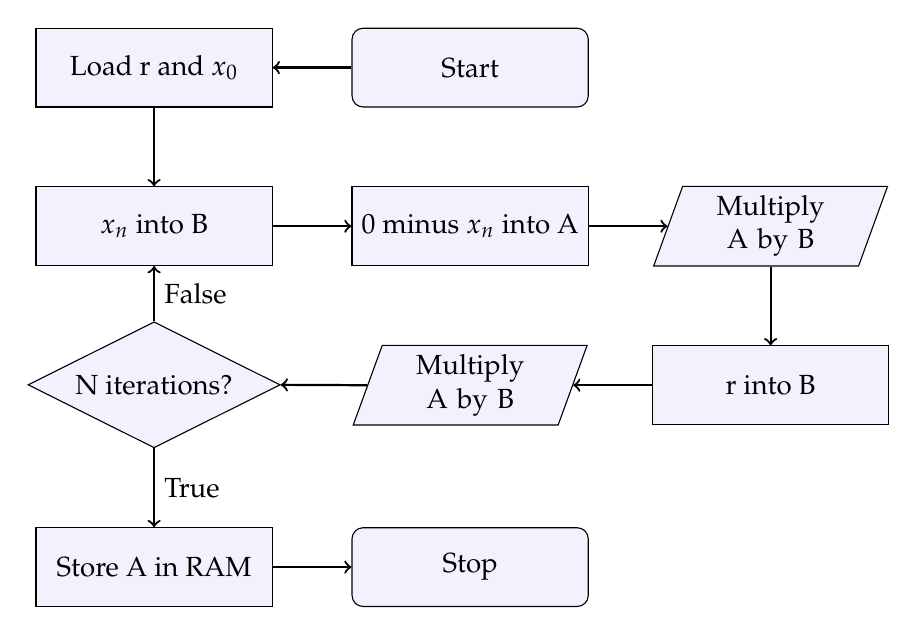
\begin{tikzpicture}
            \node[startstop] (start) {Start};
            \node[process]  (load)  [left=of start ] {Load r and $x_0$};
            \node[process]  (ldB)   [below=of load ] {$x_n$ into B};
            \node[process]  (sub)   [right=of ldB  ] {0 minus $x_n$ into A};
            \node[function] (mult1) [right=of sub  ] {Multiply A by B};
            \node[process]  (ldR)   [below=of mult1] {r into B};
            \node[function] (mult2) [left=of ldR   ] {Multiply A by B};
            \node[decision] (loop)  [below=0.7cm of ldB ] {N iterations?};
            \node[process]  (str)   [below=of loop ] {Store A in RAM};
            \node[startstop](stop)  [right=of str  ] {Stop};

            \draw[->, thick] (start.west) -- (load.east);
            \draw[->, thick] (load.south) -- (ldB.north);
            \draw[->, thick] (ldB.east) -- (sub.west);
            \draw[->, thick] (sub.east) -- (mult1.west);
            \draw[->, thick] (mult1.south) -- (ldR.north);
            \draw[->, thick] (ldR.west) -- (mult2.east);
            \draw[->, thick] (mult2.west) -- (loop.east);
            \draw[->, thick] (loop.north) -- (ldB.south) node [midway,right] {False};
            \draw[->, thick] (loop.south) -- (str.north) node [midway,right] {True};
            \draw[->, thick] (str.east) -- (stop.west);
        \end{tikzpicture}}
    \end{center}
    \caption[Logistic Map program diagram]{Program Diagram for $x_n = r \cdot x_{n-1} (1-x_{n-1})$}
    \label{fig::LogisticMapDiagram}
\end{figure}

The way that a decimal is represented limits its use to values between 0 and 1 which means that, in the simulation of the model, the population will always eventually die. To test the program, two different initial conditions with $r = 0.875$ were chosen and each was iterated 5 times. Figure \ref{tab::LogMapResults} shows $x_n$ at each iteration in both binary and decimal representation, as well as the actual value in decimal. Already after 3 iterations the error has risen above 10\% in both cases, and after 5 iterations above 35\%, which is an unfortunate limitation when using only 8 bits. Nevertheless, the results show that the program does work as intended and can evaluate the Logistic Map expression.

\begin{table}[h]
    \caption[Logistic Map program output]{Output and relative error per iteration, along with the exact values from a calculator. Base of the number is indicated by subtext. r = 0.875 and initial conditions of 0.5 and 0.25}
    \label{tab::LogMapResults}
    \begin{center}
        \begin{tabular}{lllll}
            N & Result$_2$ & Result$_{10}$ & Exact$_{10}$ & Relative Error\\\hline
            0 & 10000000 & 0.5 & 0.5 & 0\%\\\hline
            1 & 00101011 & 0.21875 & 0.21875 & 0\%\\\hline
            2 & 00111000 & 0.140625 & 0.149536 & 5.959\%\\\hline
            3 & 00011001 & 0.097656 & 0.111278 & 12.24\%\\\hline
            4 & 00010001 & 0.066406 & 0.086533 & 23.26\%\\\hline
            5 & 00001011 & 0.042969 & 0.069165 & 37.87\%\\\hline\\
        \end{tabular}
        \begin{tabular}{lllll}
            N & Result$_2$ & Result$_{10}$ & Exact$_{10}$ & Relative Error\\\hline
            0 & 01000000 & 0.25 & 0.25 & 0\%\\\hline
            1 & 00101010 & 0.164062 & 0.164062 & 0\%\\\hline
            2 & 00011100 & 0.109375 & 0.120000 & 8.856\%\\\hline
            3 & 00010101 & 0.082031 & 0.092401 & 11.22\%\\\hline
            4 & 00001110 & 0.054687 & 0.073380 & 25.47\%\\\hline
            5 & 00001000 & 0.03125 & 0.059496 & 47.48\%\\\hline
        \end{tabular}
    \end{center}
\end{table}

\section{Specifications}
\begin{table}[h!]
    \caption{Specifications of the CPU}
    \label{tab::specs}
    \begin{center}
        \begin{tabular}{l @{\quad} l}
            Clock & 0.16Hz or 6.2s per Cycle \\
            Storage & 256 bytes \\
            Architecture & 8-bit \\
            Registers & 14 General Purpose Registers \\
            Instruction Set & See Table \ref{tab::InstructionSet} \\
            I/O Ports & One input, one output \\
        \end{tabular}
    \end{center}
\end{table}

\section{Limitations and Improvements} 

\subsection{The Instruction Design} \label{ssec::InstructionLayout}
The current instruction encoding comes from an earlier prototype of the CPU and is quite outdated. As a reminder, an instruction is built up in 2 bytes, from the most significant bit to the least, as follows: four bits for the A register, 4 bits for the instruction code, four bits for the B register and four bits for the result register, where A and B can be combined to make up an immediate, an 8-bit integer encoded in the instruction. In the earlier prototype, this was done only to make wiring from the Instruction Register to the Registers easier. Since it was a very simplified setup and the programs were both tiny and programmed by placing blocks to represent the ON bits. Unfortunately, this design is very hard to read or program by hand in machine code, since A is in a different byte than B, making immediates unwieldy, and the result is in a different byte than the instruction code, making it hard to quickly parse. This does not translate directly from Assembly code to machine code and requires the reader to perform mental gymnastics jumping around within the line to parse the instruction. An improved version would arrange the four segments into their proper order: Instruction, Result, A and B. The comparison between the two design variations can be seen in Figure \ref{fig::InstrDesignComp}, where the instruction \textbf{LDA 0r3 0d100} is written out in machine code. Where beforehand an immediate was formed by A being the minor and B the major part, the roles are now reversed. This reads exactly like the assembly code and is a lot faster to parse and understand each instruction. If one would never need to interact with the binary machine code and use only assembly or a higher level language, which is possible with the completed CPU, then this problem would have no meaning to the user. However, to debug the design and function of the CPU this instruction encoding is, without understating it, a nightmare to work with.
An additional feature of this improved design is the way a program could modify itself or write its own program, since the values are in more sensible locations. A use case for this is storing variables by editing immediates to be used in the program as an argument, like a register pointer. To do this with the current design means having to be aware of the entire instruction that is meant to be modified, and then performing some bit manipulations to assemble the instruction.

\begin{figure}[ht]
    \begin{center}
        \begin{tabular}{c@{\,}cc@{\,}c|c@{\,}cc@{\,}c}
            $\overbrace{0100}^{A}$ & $\overbrace{0001}^{Instr}$ & $\overbrace{0110}^{B}$ & $\overbrace{0011}^{Res}$ & $\overbrace{0001}^{Instr}$ & $\overbrace{0011}^{Res}$ & $\overbrace{0110}^{A}$ & $\overbrace{0100}^{B}$ \\
            \textbf{4} & \textbf{LDA} & \textbf{96} & \textbf{3} & \textbf{LDA} & \textbf{3} & \multicolumn{2}{c}{\textbf{100}}
        \end{tabular}
    \end{center}
    \caption[Instruction Design Comparison]{Comparison between current design (left) and improved design (right)}
    \label{fig::InstrDesignComp}
\end{figure}

\subsection{Hard-coded Pointer}
Pointers are a big deal for programmers and software engineers that work with some lower level, more classic languages like C or C++. In Assembly, they are potentially even more important, although they are used in quite a different way. To store a value from a register into memory, the location for the variable to be stored is hard-coded into the instruction itself. If that value needs to be changed during runtime, e.g. to write values into sequential memory slots like in a list or a stack, then the actual instruction would need to be changed for the new values. A simple fix would be to have a register dedicated to acting as a pointer to write into memory. The memory module would then accept only this register as its input address during runtime. To modify the write location only this register would need to be modified, which is done the same as setting the value for any other register. Another use case would be to have a mostly-software data reader interacting with an I/O port rather than having a machine that externally controls the writing of data.

\subsection{Stack}
An important feature, if one is used to writing in assembly, that is missing, is the stack. With the aforementioned improvements, namely the hard-coded pointer, this could be solved programmatically already, but it does add a not insignificant amount of instructions to each push and pop operation. Therefore, a built-in stack module would be an improvement to the CPU, as long as it does not significantly impact the already long clock cycle. This could be achieved in a very similar way the program counter was implemented and adding push and pop operations to the instruction set, which would automatically increment or decrement the stack pointer. The stack has an incredible amount of uses, probably the biggest of which is in function calls, where e.g. the return address or arguments would be pushed to the stack and then retrieved when needed. Additionally, this would decrease the need for more than a few registers, since variables could be pushed and popped from the stack, as it is commonly done in Assembly.

\subsection{Complexity}
The layout of the CPU is far from optimal and leaves a lot of room for improvements. Most importantly, the wiring needs to be cleaned up and smoothed out, because especially the gap between the RAM and the CPU is incredibly messy. Many wires need to switch levels, some going on the upper level and others going on the lower level, all while crossing each other in numerous instances. A few iterations on the layout and wiring itself could probably drastically reduce the messiness and make the wiring look more appealing to the eye.

Furthermore, the implementation of the clock is unnecessarily complicated and involves a series of uncomfortable workarounds to function properly. It makes abundant use of Minecrafts timing functionality to reach a certain component at a very specific time, rather than being solved logically and, very importantly, more reliably. For example, the flags register gets updated by the ALU after it completed its operation. In order to store the flags, a pulse from the clock is required, which, to compensate for the time the ALU takes to calculate, is delayed significantly. A solution would be to use a flip-flop, as it was suggested in the Danger Sign Problem (See section \ref{ssec:DangerSign}) and simply write to the flags register at the next clock pulse.

\chapter{Appendix}

\label{Appendix}

\section{Resources}
\subsection{8bit-CPU-Minecraft Repository} \label{app::Repository}
All the programs and the world file are in the repository as of 06.01.2024.

https://github.com/DantezMine/8bit-CPU-Minecraft

\section{Code}
\subsection{Assembler} \label{app::Assembler}
\lstinputlisting[language=Python]{Code/Assembler.txt}

\subsection{Binary To Schematic} \label{app::BinarySchem}
\lstinputlisting[language=Python]{Code/BinarySchem.txt}

\section{Programs}
\subsection{Fibonacci} \label{app::Fibonacci}
\lstinputlisting[language=Python]{Code/Fibonacci.txt}

\subsection{Multiplication} \label{app::Multiplication}
\lstinputlisting[language=Python]{Code/Multiplication.txt}

\subsection{Logistic Map} \label{app::LogisticMap}
\lstinputlisting[language=Python]{Code/LogisticMap.txt}


\printbibliography[title=Sources]

\listoffigures % Prints the list of figures

\listoftables % Prints the list of tables

%----------------------------------------------------------------------------------------
%	DECLARATION PAGE
%----------------------------------------------------------------------------------------

\begin{declaration}
	\addchaptertocentry{\authorshipname} % Add the declaration to the table of contents
	\noindent Der/die Unterzeichnete bestätigt mit Unterschrift, dass die Arbeit selbständig verfasst und in schriftliche Form gebracht worden ist, dass sich die Mitwirkung anderer Personen auf Beratung und Korrekturlesen beschränkt hat und dass alle verwendeten Unterlagen und Gewährspersonen aufgeführt sind.
	\vspace{1.5cm}
	
	\noindent Unterschrift:\\
	\rule[0.5em]{25em}{0.5pt} % This prints a line for the signature
	
	\noindent Ort/Datum:\\
	\rule[0.5em]{25em}{0.5pt}\\ % This prints a line to write the date
	(aus den Richtlinien zur Maturitätsarbeit, S.6)
	\end{declaration}

\end{document}